\chapter{Feature Engineering}
\label{ch:feature_engineering}
The ultimate goal of `Feature Engineering' is to clean and transform the data
using heuristics and event tagging. Events are tagged to identify tracks which
are likely to originate from signal sources, as separate from events which come
from the background. Subsequently, the signal to background ratio and
longitudinal spin asymmetry are measured.

Even with the Forward Upgrade (Section~\ref{sec:forward_upgrade}), the data set
is still composed mostly of background events. The primary constituents of the
data set are muons from the following sources:

\begin{itemize}
  \item \textbf{Hadronic Background}
    \begin{itemize}
      \item This hadronic background source is composed of hadrons which are
        produced at the primary event vertex, and then travel into the Muon
        Arms. The hadrons then decay into muons in the volume of the Muon Arms.
        The hit pattern from such decays is mis-reconstructed as high-$p_T$
        muons originating at the primary event vertex. Though the probability of
        this scenario is small, the large number of hadrons results in a
        substantial background. 
    \end{itemize}
  \item \textbf{Muon Background}
    \begin{itemize}
        \item The muon background is composed of processes which produce real
          muons which fall into a similar kinematic regime of the W-genic muons.
          This contribution is separated from the signal data set with a
          combination of likelihood event tagging (Section~\ref{sec:likelihood})
          and an unbinned maximum likelihood fit (Section~\ref{sec:sbr}).
    \end{itemize}
  \item \textbf{W Signal}
    \begin{itemize}
        \item These are the original muons from the $W$ Boson decay, and carry
          information about the proton's spin.
    \end{itemize}
\end{itemize}

Likelihood event selection is applied in the first stage of event selection,
where two classifications are considered for muon tracks. The first
classification is `background', which is composed of real muon background, and
mis-reconstructed muon tracks originating from hadronic decay. The second
classification is `signal', which is composed of muons which have a high
likelihood of having decayed from a $W$-Boson, alternatively referred to as
`W-genic' tracks. This process is described in Section~\ref{sec:likelihood}.

The second stage of event selection differentiates the data set into three
classifications--hadronic background, muon background and $W$-Boson decays.
The recorded data set is used as a proxy for the hadronic background, while the
$W$ Boson and Muon Background contributions are modeled with a combination of
simulation of tracks originating from the $W$ Boson and Muon Background
processes, as well as extrapolation from the data set. This is accomplished with
a Maximum Likelihood Fit, described in Section~\ref{sec:sbr}.

In subsequent sections, I will provide a greater context for motivating the
selection of analysis variables. As this data set is dominated by background
sources, the analysis relies heavily on simulations to estimate how signal $\mu$
events might look like in the PHENIX detectors.

At the time of writing, simulation of hadronic background has not yet been
incorporated into the analysis, as there are many effects to consider. For
example, how particles interact with the material of PHENIX to produce secondary
and tertiary vertices. Also, as the percentage of hadronic background events
which mimic W-genic muons is very small, trillions of events need to be
generated. However, it is possible to accurately simulate the signal process,
and the muon background processes, since both know these processes are
understood with high precision.

To form the basis of separating signal and background, the data itself is used
as a proxy for what the `hadronic background' may look like, and the simulations
are used to represent the portions of data which cannot come from this hadronic
background. Even so, it is certain that the $W$ signal must be in the data
sample.

\clearpage
\section{The Basic Cut}
\label{sec:basic_cut}

The basic cut aims to remove all events which are kinematically forbidden from
resulting from a $W$-boson decay. Because the $W$ boson must produce narrowly
curved muons due to high momentum, one may remove tracks outside of a momentum
threshold. The threshold is defined both in terms of the actual reconstructed
momentum, as well as with respect to variables which are correlated to the
amount of track bending.

{\noindent}The ``Basic Cut'' is defined:
\begin{table}[ht]
  \centering
  \begin{tabular}{l c c}
    \toprule
    \textbf{Variable} & \textbf{Lower Bound} & \textbf{Upper Bound} \\
    \midrule
    DG0 & 0 $cm$ & 20 $cm$ \\
    DDG0 & 0.0 $^\circ$ & 9.0 $^\circ$ \\
    DCA$_r$ & 0 $cm$ & 30.0 $cm$ \\
    $\chi^2$ & 0 & 20 \\
    $p$ & 5 $GeV/c$ & 250 $GeV/c$ \\
    $p_T$ & 16 $GeV/c$ & 60 $GeV/c$ \\ 
    $RPC_1DCA$ & 0 $cm$ & 20 $cm$ \\
    $RPC_3DCA$ & 0 $cm$ & 40 $cm$ \\
    $fvtx_{d\theta}$ & 0 $rad$ & 1.5 $rad$ \\
    $fvtx_{d\phi}$ & 0 $rad$ & 1.5 $rad$ \\
    MuID lastGap & Gap 4 & * \\ 
    Number of $\mu$ Tracks Per Event & N/A & 1 \\
    \bottomrule
  \end{tabular}
  \caption{ 
    The Basic Cuts used in the Run 13 analysis. lastGap refers to the last gap
    in the MUID which saw a $\mu$ candidate event. The fourth gap is the
    furthest penetration possible, therefore suggesting a high enough energy
    muon.  Other parameters are described in Tables \ref{tab:evt_variables},
    \ref{tab:mutr_variables}, \ref{tab:fvtx_variables}, and
    \ref{tab:rpc_variables}
  }
  \label{tab:basic_cut}
\end{table}

With this cut, a we reduce the background in our data by a factor of about
15,700--without worry of removing any events in that fall within the kinematic
range of $W$ Boson production. The basic cut reduces our data set from 15.7
billion events to about one million events.

\clearpage
\section{Simulations}
\label{sec:simulations}

PHENIX has a rather well developed simulation framework, which uses the in-house
built ``PHENIX Integrated Simulation Application'' (PISA)~\cite{Maguire1997}
custom simulation framework. The simulation framework models the entire
12m$\times$18m$\times$18m volume of the PHENIX apparatus in detail, as well as
all the various material properties of the apparatus. The software package uses
GEANT as a basis, with PHENIX geometry build on top. PISA additionally
encapsulates event-generators, a standalone geometry verification package, and
the PHENIX offline analysis shell, in order to generate data that is completely
compatible with PHENIX's data packaging framework. PISA has since been
integrated into a simulation work-flow with the standard-bearing PYTHIA event
generation system.

The simulations were created by selecting the biggest sources of muon background
produced at PHENIX as predicted by the Standard Model as well as the $W$ Boson
event. Events were generated until a large enough sample was accumulated to
provide statistically significant distributions of simulated data.

The purpose of simulating the muon background and W-Signal is to generate
probability distribution functions for the variables which have the largest
analyzing power--i.e. ability to differentiate between signal and background.

After producing a simulated data set, the simulations for muon background were
summed to produce a data set to represent what a data set composed only of these
processes might look like. The yields of each process were normalized to
represent the actual fraction of the total data set that each process
contributed, which is summarized in Table~\ref{tab:simulation_cross_sections}.
The simulation for the $W$ Boson muon decay was treated similarly, but kept
separate from the muon background.

Along with our proxy for the hadronic background, extracted from the real data
set, we produce probabiltiy distribution functions for each variable used in the
analysis in order to facilitate the likelihood event selection.

For the simulations, we consider the following processes: Open charm or
charmonium refers to the bound state of the $c\bar{c}$ quarks. The Onium muon
background source refers to any process where a quark is in a bound-state with
its own antiparticle, excluding $c\bar{c}$ and $b\b{bar}$ which is simulated
separately. Open bottom refers to the bound state of $b\bar{b}$ quarks.
Z/$d\gamma$ refers to the production and decay of the mixing between the Z-boson
and virtual photons. ONLY Z refers to Z production and decay.  W is the signal
event in this work.  These processes are summarized in
Table~\ref{tab:simulation_cross_sections}.  

\begin{table}[ht]
  \centering
  \begin{tabular}{ccccc}
    \toprule
    \multicolumn{5}{c}{\textbf{Reference Run 393888}}\\ 
     & & & & \\
    \textbf{Process} & 
    \textbf{k factor} & 
    \textbf{$\sigma$ } & 
    \textbf{\# Events} & 
    \textbf{ $\mathcal{L}$ } \\
    & & (\textit{mb}) &  & ($fb^{-1}$) \\
    \midrule
    $c\bar{c}$ & 2.44  & 5.71e-01 & 5.85e+11 & 1.02 \\
    onium      & 0.415 & 1.35e-01 &  1.5e+11 & 1.11 \\
    $b\bar{b}$ & 1.83  & 7.30e-03 & 7.36e+09 & 1.01 \\
    ONLY Z     & 1.25  & 3.37e-07 & 1.73e+08 & 577.0\\
    W          & 1.5   & 1.66e-06 & 3.38e+08 & 198.9\\
    Z          & 1.25  & 1.02e-06 & 2.93e+08 & 61.2 \\
    \bottomrule
  \end{tabular}
  \caption{
    Simulated sub processes in Run 13 including their generated event numbers as
    well as the corresponding luminosity and cross sections.  An extensive
    analysis of the simulated data was undertaken to determine an appropriate
    k-factor. 
  }
  \label{tab:simulation_cross_sections}
\end{table}                  
``

The simulations must additionally be weighted for trigger efficiency. To
accomplish this, we weight events for each arm and charge with the associated
trigger efficiency when constructing probability density functions representing
the muon background. The trigger efficiencies generally manifest as $\eta$
dependent functions--thus we bin the data into 20 separate $\eta$ bins and
calculate the efficiency associated with each bin. The bin ranges, and
efficiency corrections are summarized in
Table~\ref{tab:rapidity_corrections_north} for the North arm, and
Table~\ref{tab:rapidity_corrections_south} for the South arm in the appendix.

The trigger efficiencies of the archived data is needed in order to correct the
overall yields of events in the data-set, and is done by scaling the yield of a
particular trigger with the efficiency. This analysis was presented
in~\cite{Seidl2014a}.

One can visualize the composition of the simulated data set by stacking the
relative distributions of these variables. Observing the cross-sections of these
variables as a function of $p_T$, allows one to see how the background
composition varies with $p_T$ (Figure~\ref{fig:stacked_xsec_sim}).

\begin{figure}[ht]
  \centering
  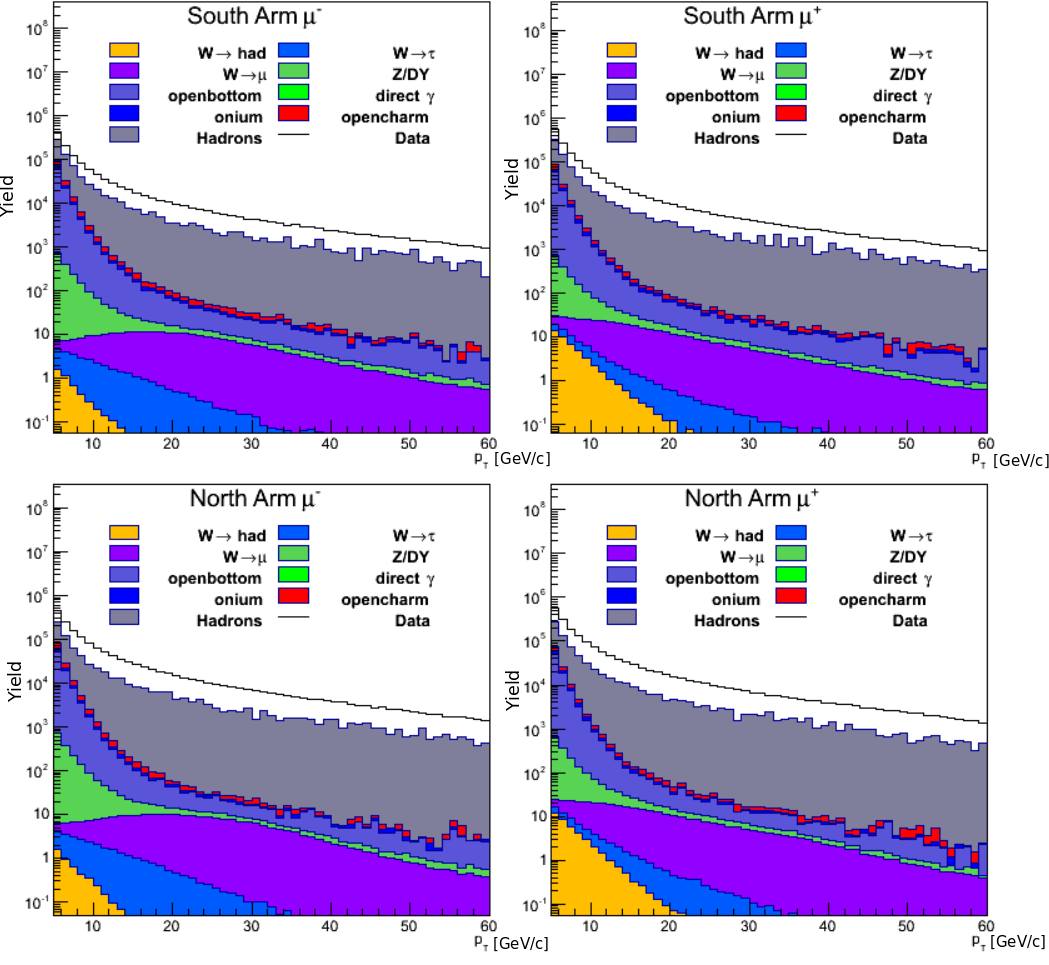
\includegraphics[width=\linewidth]{./figures/stacked_xsec.png}
  \caption{
    Shown: stacked cross-sections of all simulated processes as a
    function of $p_T$. All data shown has been created from the PISA+PYTHIA
    framework. Top Left: South $\mu-$, Top Right: South $\mu+$, Bottom Left:
    North $\mu+$, Bottom Right: North $\mu-$~\cite{Seidl2014a}
  }
  \label{fig:stacked_xsec_sim}
\end{figure}

\clearpage


\section{$W_{ness}$: Likelihood Event Tagging}
\label{sec:likelihood}

Recalling that the dataset into is already split into three main contributions:
hadronic background, real muon background, and W-Signal, the next task is to 
formulate a means to separate signal from background.

Previous analyses have attempted to separate the muon spectrum into $p_T$ bins,
to estimate the composition, however, because the $W\rightarrow\mu$ signal is so
small in the forward kinematic regime, these methods are not viable, as
there is no `visible' cutoff in the spectrum associated with a invariant mass
peak at half the mass of the $W$ Boson.

High momentum $\mu$ tracks are straight, with less bending then other $\mu$
tracks. The kinematic variables describing track reconstruction have
characteristically narrow distributions for our signal muons.

One can think of the study of the data set in terms of a classification problem.
Bayes Theorem is at the foundation of a robust classification technique, known
Naive Bayes. Using this technique to classify a data requires that one has a
sample of labeled testing data to construct a model which can classify data into
two or more classes. Care must be taken not over-train the classifier, or
attempt to classify data which has been used in the subset of data to train the
classifier. An example of over-training might be a case where one customizes the
model by providing training data which is not representative of the real
variation in the true data set, which artificially inflates the model's
accuracy when used on training data.

In this case, simulations serve as the training data, guaranteeing that there
will be no overlap between the physical data produced, and the data used to
train the classifier. Thus, a Naive Bayes Classifier is implemented (also known
as Likelihood Selection) to label our data with two classes. Rather than
labeling data with a binary classification, data is labeled with its likelihood
of receiving a `signal' classification.

\subsection{Naive Bayes Classification}

There are many techniques available for classifying a collection of variables (a
feature set) into categories. Naive Bayes is  useful in cases where meaningful
classification categories can be applied to feature sets, and labeled training
data is available. One advantage of Naive Bayes is that after training the
classifier, very large data sets can be classified, with little computational
resources needed to store the classifier itself. A soft requirement for Naive
Bayes classification is that feature sets must not be correlated, since this can
lead to over training. Originally used for classification of text documents,
Naive Bayes is also able to handle numeric features whose distributions are
known~\cite{Collins2013}.

In this analysis, consider our track reconstruction variables as the `feature
set', and the classification of `signal' or `background' as the label.

In order to obtain the best performance from the classifier, without
over-training, one must ensure that the variables used to determine a class are
maximally uncorrelated. The variables which match this criteria are: DG0, DDG0,
$\chi^2$, $fvtx$ variables, Rpc1DCA, Rpc3DCA, DCA$_r$, and DCA$_z$. The linear
correlations between these variables are shown for both the data, and the
simulated W-Signal in Figure~\ref{fig:kinematic_var_correlations}.

\begin{figure}[H]
	\centering
	\begin{subfigure}[t]{0.5\textwidth}
		\centering
		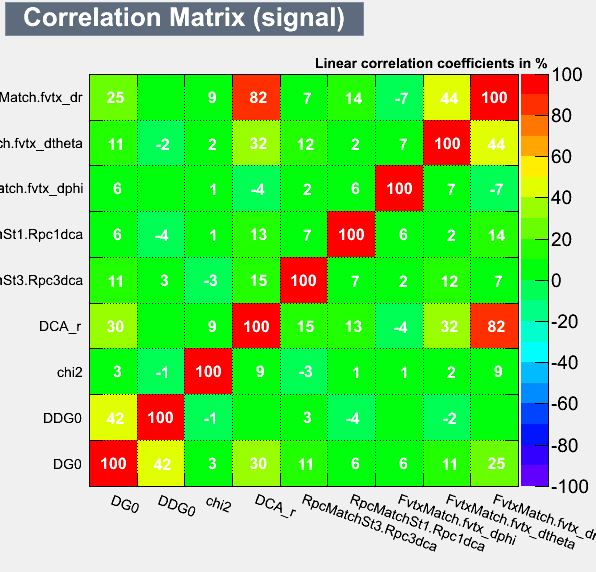
\includegraphics[width=0.95\linewidth]{./figures/CorrelationMatrix_Signal.png}
		\caption{
      Simulated $W$ Boson $\mu$ events
    }
		\label{fig:corr_mat_sig}
	\end{subfigure}%
  \begin{subfigure}[t]{0.5\textwidth}
		\centering
		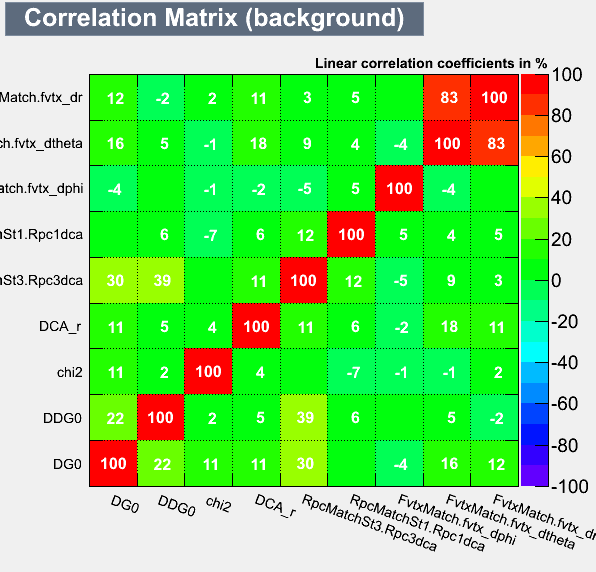
\includegraphics[width=0.95\linewidth]{./figures/CorrelationMatrix_Background.png}
		\caption{
      Real data proxy for hadronic background
    }
		\label{fig:corr_mat_bkg}
	\end{subfigure}
	\caption{ 
    In panel (a) Correlations are shown between kinematic variables, produced
    from the signal simulation. In panel (b) correlations are shown for the real
    data proxy for hadronic background. Variables that are correlated are
    combined in two dimensional probability distribution functions, i.e. DG0 and
    DDG0 and DCA$_r$ and $\chi^2$.
    }
	\label{fig:kinematic_var_correlations}
\end{figure}

As one can see from Figure~\ref{fig:kinematic_var_correlations}, DG0 and DDG0
are slightly correlated, as are $\chi^2$ and DCA$_r$. A Naive Bayes classifier
may be constructed from the core of the familiar Bayes Theorem from probability
and statistics. In our case, we understand Naive Bayes as a conditional
probability. Concretely, we consider a vector of features (i.e.  our
discriminating kinematic variables):

\begin{equation}
	\label{eq:feature_vector}
\mathbf{x} = (x_1, \dots, x_n)
\end{equation}

{\noindent}and assume independence between each feature $x_n$. We then define the
probability of a given classification, $C_k$ (i.e. signal or background) given a
set of features $x_n$ (i.e. DCA$_r$, $\chi^2$ ...):

\begin{equation}
	\label{eq:cond_probabilty}
  \mathcal{P}(C_k \vert x_1, \dots, x_n)
\end{equation}

{\noindent}This conditional probability is defined in terms of Bayes Theorem:

\begin{equation}
	\label{eq:bayes_theorm}
  \mathcal{P}(C_k \vert \mathbf{x}) = \frac{\mathcal{P}(C_k) \
  \mathcal{P}(\mathbf{x} \vert C_k)}{\mathcal{P}(\mathbf{x})}
\end{equation}

{\noindent}The terms here are defined as:
\begin{itemize}
  \item $\mathcal{P}(C_k)\rightarrow$ prior probability
	\item $\mathcal{P}(\mathbf{x} \vert C_k)\rightarrow$ likelihood
	\item $\mathcal{P}(\mathbf{x})\rightarrow$ overall probabiltiy
\end{itemize}

The probabilities described here are realized through constructing probability
density functions from the data and simulations. The constraints for choosing
PDFs to use represent the two lables are: (1) PDFs must be able to be
meaningfully normalized, (2) PDFs associated with each label should have a
unique enough shape to differentiate between either label, and (3) the PDFs
should be uncorrellated.
 

The likelihood ratio is constructed using the posterior probability
for each classification, which is defined as $W_{ness}$:
\begin{align}
  \lambda_{sig} &= \prod_{k}\mathcal{P}(\mu_{sig}\vert C_k)\\
  \lambda_{bak} &= \prod_{k}\mathcal{P}(\mu_{bak}\vert C_k)\\
  W_{ness} &= { 
    {\lambda_{sig}}
    \over 
    {\lambda_{sig}+\lambda_{bak}}\label{eq:wness_calculation}
  }
\end{align}

{\noindent}Where $\lambda_{sig}$ and $\lambda_{bak}$ represent the total
likelihoods that a given track is either signal, or background, constructed from
the product of likelihoods calculated from each probability density function.

{\noindent}$\lambda$ is the final product of the componant probability
distribution functions:

\begin{equation}
	\lambda =
	p(DG0,DDG0)p(\chi^2)p(DCA_r)p(RPC1/3DCA)p(fvtx_{dr})p(fvtx_{d\theta})p(fvtx_{d\phi})
	\label{eq:full_lambda}
\end{equation}

Note that the PDFs are composed by creating a histogram of the synonymous
kinematic variable associated with the label of `signal' or `background'. In the
case of DG0 and DDG0, we use a 2D histogram to account for correlation, as well
as DCA$_r$ and $\chi^2$.

In order to construct probability distribution functions to use in this
classification, one must select samples of labeled data representing each
classification. The recorded data is used as a proxy the `background' labeled
data set, and the simulation of the $W$ boson decay is the `signal' labeled data
set. The $W$ Boson signal at this stage of the analysis does not meaningfully
change the shape of the PDFs extracted from the data. Even after the Basic Cut,
the number of $W$ Boson decay events is small relative to the hadronic and muon
background (less than one part in 1000). The $W$ Boson production cross section
is precisely known--since the luminosity delivered to PHENIX is also known, the
$W$ Boson yield may be trivially estimated.

Not all recorded events contain valid tracking information for all tracks. For
example, consider a muon track which was recorded due to a minimum bias trigger.
When any trigger causes data to be recorded, there is no guarantee that all
subsystems have been triggered, but all subsystems flush the data in their
buffers to the archival data stream. This is not an error, each detector
subsystem has an associated efficiency and acceptance.  For example, with our
example track, perhaps the physical process related to triggering a detector
simply didn't occur. One may correct account for all this when constructing
PDFs.  A selection process is superimposed such PDFs are constructed only from
events (simulated or otherwise) containing valid data. Similarly, the selection
process must also be preserved when looking up what PDFs to ultimately use in
calculating the likelihood of an event being generated from a signal process.
This process is represented in Figure~\ref{fig:pdf_selection_tree}.

\begin{figure}[ht]
  \centering
  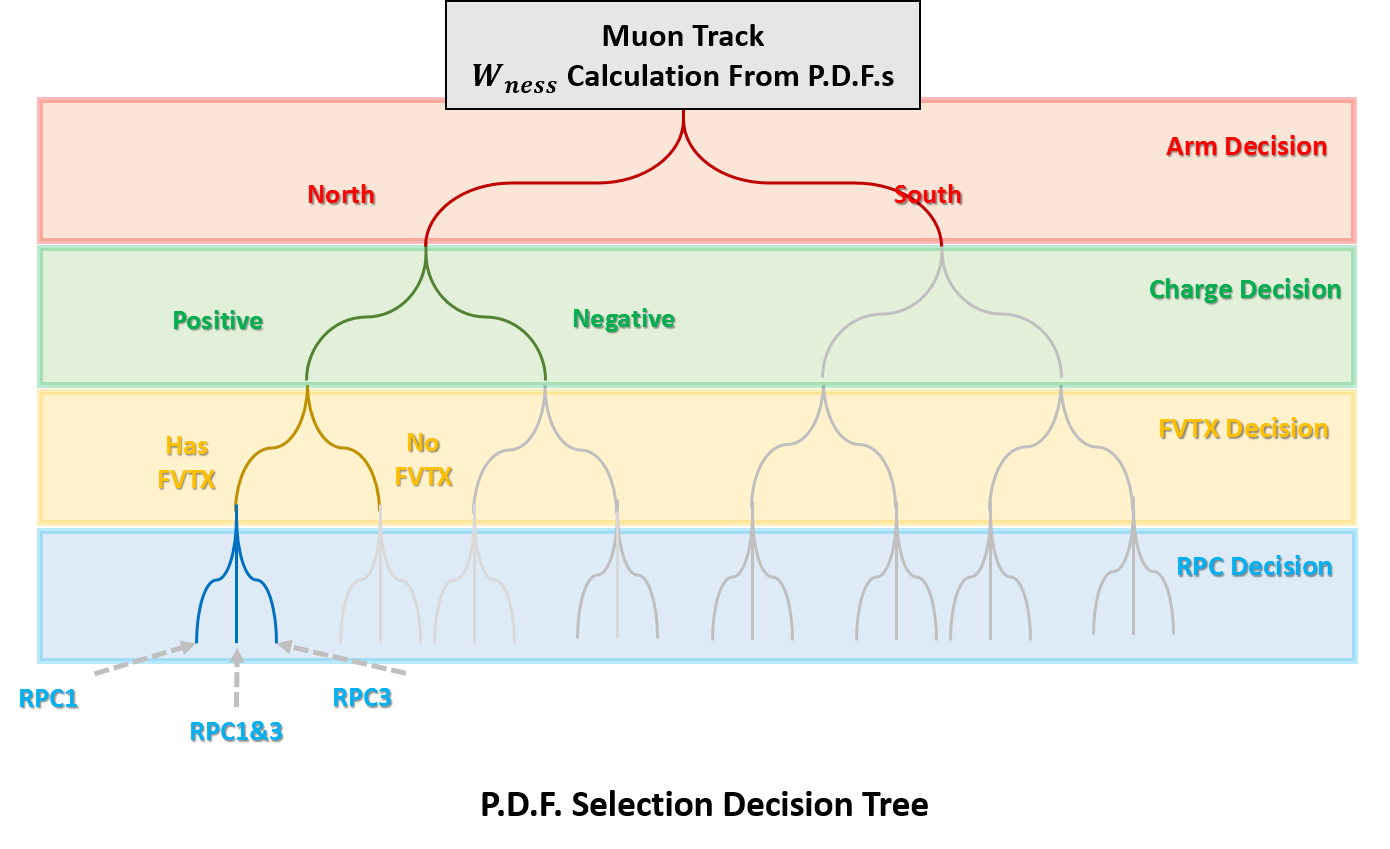
\includegraphics[width=\linewidth,trim=4 70 4 4,clip]{./figures/pdf_selection_tree.png}
  \caption{
    A cartoon of the decision tree to determine the PDF cocktail to use for
    quantifying the $W_{ness}$ of a given track. The track's properties are used
    to traverse the tree, and select the cocktail contents.
  }
  \label{fig:pdf_selection_tree}
\end{figure}

Finally, once all PDFs have been constructed, following the selection process
shown in Figure~\ref{fig:pdf_selection_tree}, one may loop over the simulated
data set, and the recorded data set, and perform the likelihood calculation for
each muon track (Equation~\ref{eq:wness_calculation}). The value of
$W_{ness}$ is stored for every track in the simulation and data as an
engineered feature to be used in cuts.

In figures~\ref{fig:pdf_rpc3dca}-\ref{fig:pdf_DG0}, the probability
distribution functions are shown for each arm and charge combination. In the
figures, we represent the product of all probability functions which are used
to tag an event as $\lambda$ such that $\lambda = \Pi_{k} \mathcal{P}(\mu \vert
C_k)$. The 1D distributions are shown for all variables to highlight each
varaible's distribution, but recall that DG0 and DDG0 are combined into a 2D
histogram in practice, along with DCA$_r$ and $\chi^2$. As an example, the PDF
for DCA$_r$ (Figure~\ref{fig:pdf_dcar}) is shown, with the remaining PDFs
included in the appendix.

\begin{figure}[ht]
  \centering
  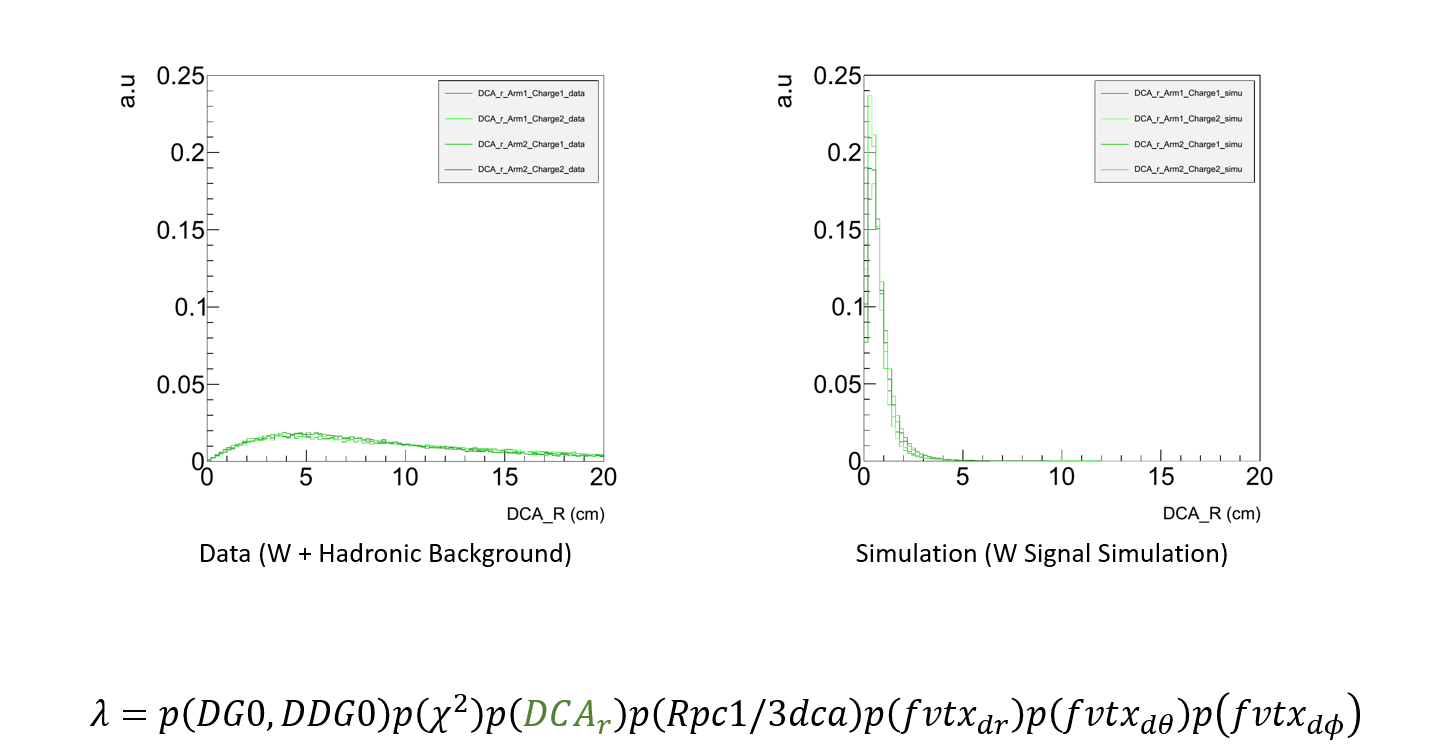
\includegraphics[width=\linewidth,trim=4 70 4 4,clip]{./figures/pdf_dcar.png}
  \caption{
		The left panel shows the distribution of DCA$_r$, the transverse distance of
		closest approach between the track and the event vertex, for each arm and
		charge, produced from the PHENIX data set, after the basic cut. The right
		panel the same distributions from a simulation of the W-Signal. Both panels
		have the arm and charge data partitions overlaid.
  }
  \label{fig:pdf_dcar}
\end{figure}

After constructing PDFs, the $W_{ness}$ is calculated for each muon track
(Equation~\ref{eq:wness_calculation}) contained in the recorded data set, and
the simulated data set for the $W$ Boson signal.  The final distributions of
$W_{ness}$ are shown for signal simulation and the recorded data in
Figure~\ref{fig:wness_distribution}.

\begin{figure}[ht]
  \centering
  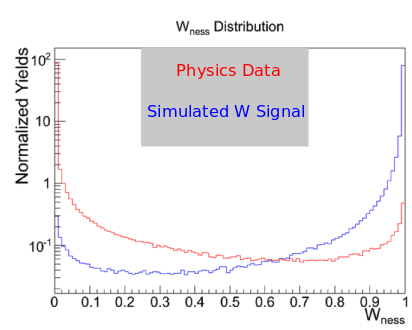
\includegraphics[width=0.7\linewidth]{./figures/wness_sig_bak.png}
  \caption{
		Distributions of $W_{ness}$ are shown for the recorded data in red, and the
		simulated data in blue. Note that the vertical is plotted on a log scale.
		The two distributions have been normalized to total area. 
  }
  \label{fig:wness_distribution}
\end{figure}

As seen in Figure~\ref{fig:wness_distribution}, most of the simulated data falls
in the high $W_{ness}$ range while most of the physics data falls in the low
$W_{ness}$ range. The goal of the likelihood analysis is to tag the data with
$W_{ness}$ in order to apply cuts on the data based on the likelihood. The cut
is applied such that background is removed with minimal reduction in signal.
This is accomplished by applying successive $W_{ness}$ cuts and choosing the cut
which minimizes the reduction in potential signal events, summarized in
Figure~\ref{fig:wness_cut_efficiency}.

\begin{figure}[ht]
  \centering
  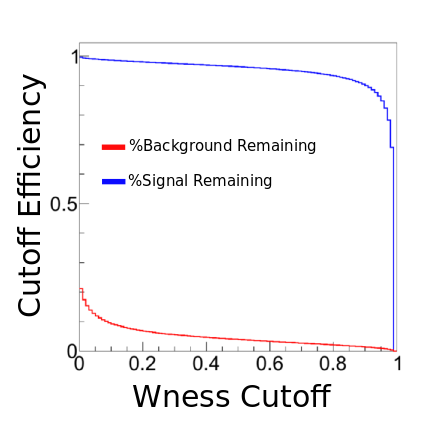
\includegraphics[width=0.7\linewidth]{./figures/wness_cut_efficiency.png}
  \caption{
		Shown: the fraction of signal and background remaining (vertical axis) in
		the total data set with successively higher cuts in $W_{ness}$ (horizontal
		axis). The inflection point in the blue distribution is chosen as the
		optimal $W_{ness}$ cut.
  }
  \label{fig:wness_cut_efficiency}
\end{figure}

To obtain optimal $W_{ness}$ cutoff, successive cuts in $W_{ness}$ are made. The
fraction of signal and background was compared at each cut. It is found that
$W_{ness} > 0.95$ (the likelihood of a track receiving the `signal' label) is
the optimum cutoff. Data below this threshold will represent the data population
containing only background events, while data above this threshold represents
the fraction of the data containing signal events.

Note that now with this reduced data set, one could simply assume that all
remaining data is signal, and calculate an asymmetry, however, there is clearly
still a lot of background present. Any background that is still present will
dilute the longitudinal asymmetry in $W$ production. Therefore, an unbinned
maximum likelihood fit (Section~\ref{sec:sbr}) is applied to the remaining data
set, in order to estimate the residual background contribution. The result of
the fit will estimate the residual fraction of Muon Background, Hadronic
Background and W-genic muons in the data after applying the $W_{ness}$ cut.  The
fit is applied over a domain of $W_{ness}$, $\eta$ and $dw_{23}$. 

\clearpage
\section{Extended Unbinned Maximum Likelihood Selection: The Signal to
Background Ratio}
\label{sec:sbr}

\subsection{Introduction}
\label{sec:sbr_intro}
The goal of the Extended Unbinned Maximum Likelihood Fit (EULMF) is to extract
the signal to background ratio, which in turn helps to estimate the background
dilution in the measurement of the longitudinal asymmetry. The EULMF is a
statistical method which relies on creating Probability Density Functions to
represent the likelihood that a given track to originates from the muon
background, $W$ signal or hadronic background. However, this is distinct from
the Likelihood Selection Method (Section~\ref{sec:likelihood}) because rather
than using likelihood to tag events, PDFs are fit to recorded data itself.
After the fits, the overall composition of the recorded data remaining after the
$W_{ness}$ cut is estimated. Yields are obtained for three categories of
data--Hadronic Background, Muon Background, and $W$ signal. 

The EULMF uses PDFs formed to represent $dw_{23}$ and $\eta$. $dw_{23}$ and
$\eta$ are uncorrelated, and are additionally uncorrelated from the PDFs used to
calculate $W_{ness}$. This helps to avoid over-fitting, especially since
$W_{ness}$ is used explicitly to facilitate the extraction of the $dw_{23}$ PDF
representing the hadronic background. 

The PDFs representing $\eta$ and $dw_{23}$ representing  $W$ signal are
extracted directly from simulations. Additional care is needed for extracting
the PDFs representing the Hadronic Background
(Section~\ref{sec:hadronic_background_pdfs}). The shape of $dw_{23}$ for
hadronic background is extrapolated from the low $W_{ness}$ portion of the
recorded data into the signal region $W_{ness} > 0.95$. $\eta$ has an unchanging
shape with respect to $W_{ness}$, therefore its shape is extracted directly from
the $W_{ness} < 0.95$ portion of the recorded data. The details of extracting
the hadronic background PDFs are discussed in
Section~\ref{sec:hadronic_background_pdfs}.

When forming the PDFs representing $dw_{23}$ and $\eta$ for the Muon Background,
the yields of each simulated process are weighted and added together to reflect
the expected composition of the Muon Background in the recorded data. The
details of extracting the PDFs from simulated data are discussed in
Section~\ref{sec:simulation_pdfs}. 

{\noindent}With PDFs generated that representing Muon Background, $W$ signal and
the hadronic background, the EULMF is defined:

\begin{equation} 
  \mathcal{L}(\theta|X) 
  \equiv
  \frac{n^N e^{-n}}{N!} \prod_{x_i \in X}^N
  \sum_c \frac{n_c}{n} p_c (x_i), \
  ;{\rm with}\, 
  n=\sum_c n_c 
  \label{eq:likelihood_function}
\end{equation} 

{\noindent}where $X$ is the sample of $N$ total events $x_i =
(\eta_i,{dw_{23}}_i)$, and $\theta$ gives the parameters of the fit $\theta =
(n_{sig},\,n_\mu,\, n_{had})$. $c$ is an index running over the three data types
(muon background, hadronic background, $W$ signal). In the fit, the Muon
Background, $n_\mu$, is fixed to the expected yields of these processes
according to the cross section of muon background processes, and machine
luminosity. The remaining parameters are obtained from the fit $(n_{sig},\,
n_{had})$ by minimizing the $-\log(\mathcal{L}(\theta|X))$. Due to the large
integrated luminosity, 277 $pb^-1$, of 2013's data set, the data was able to be
partitioned evenly into three $\eta$ bins: $1.10 < \eta < 1.40$, $1.40 < \eta <
1.80$ and $1.80 < \eta < 2.60$. The EULMF was performed with signal to
background ratios evaluated and asymmetries calculated for each bin.

\subsection{Hadronic Background PDFs}
\label{sec:hadronic_background_pdfs}
The main analysis challenge for the EULMF is describing the shape of the
hadronic background PDF associated with $dw_{23}$. Care must be taken here,
since the data set ultimately contains the desired signal events. If one takes
the data set in the signal region to be representative of the hadronic
background's shape, signal events will be severely under-counted. The task of
properly extrapolating $dw_{23}$ is accomplished by observing the shape of
$dw_{23}$ at different $W_{ness}$ values, and parameterizing the way that that
its shape changes with increasing $W_{ness}$. This is qualitatively presented in
in Figures~\ref{fig:dw23_eta_wness_dat} and~\ref{fig:dw23_eta_wness_sim}, where
a $dw_{23}$ is seen in the recorded data to slowly narrow as $W_{ness}$
increases--contrasting with the simulated distribution which is uniformly
narrow. This suggests that a broader $dw_{23}$ is more associated with hadronic
background. Conversely, the shape of $\eta$ is not as sensitive to $W_{ness}$.

\begin{figure}[ht]
  \centering
  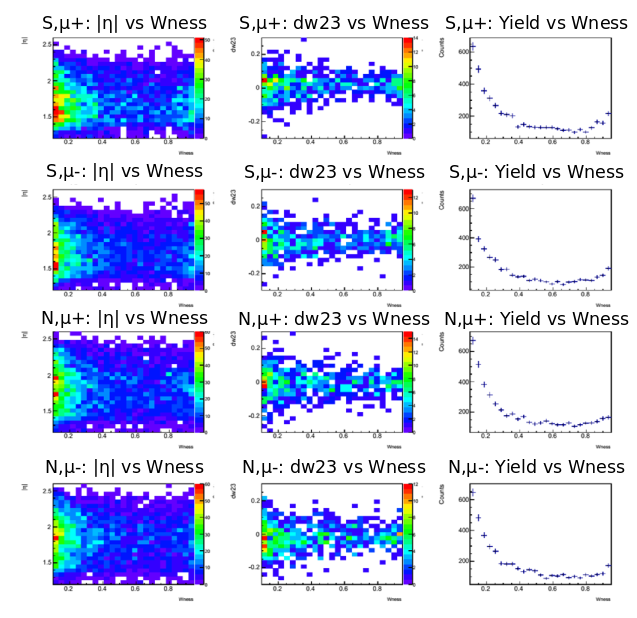
\includegraphics[width=\linewidth]{./figures/dw23_vs_wness_data.png}
  \caption{
    Shown: distributions of the recorded data set for $dw_{23}$, $\eta$ and
    $W_{ness}$.  The first column shows $\eta$ as a function of $W_{ness}$. The
    middle column shows $dw_{23}$ as a function of $W_{ness}$, and the right
    column shows a histogram of the $W_{ness}$ distribution. The rows all
    correspond to (top to bottom): North, $\mu+$, North $\mu-$, South $\mu+$,
    and North $\mu-$.
  }
  \label{fig:dw23_eta_wness_dat}
\end{figure}

\begin{figure}[ht]
  \centering
  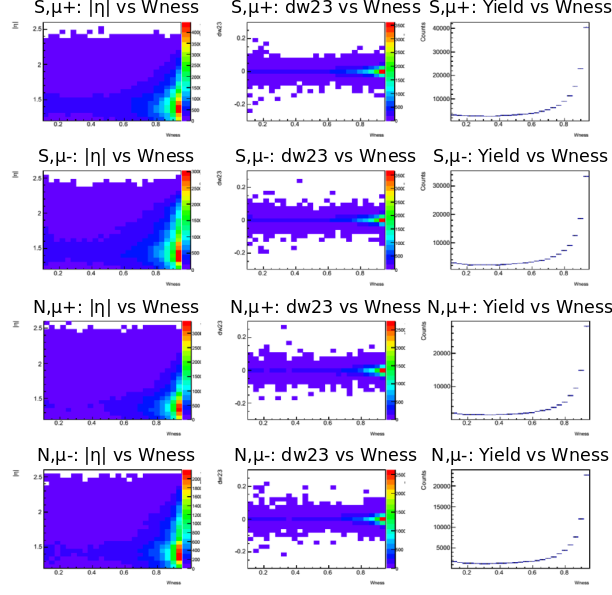
\includegraphics[width=\linewidth]{./figures/dw23_vs_wness_simulation.png}
  \caption{
    Shown: distributions of the simulated $W$ signal data set for $dw_{23}$,
    $\eta$ and $W_{ness}$.  The first column shows $\eta$ as a function of
    $W_{ness}$. The middle column shows $dw_{23}$ as a function of $W_{ness}$,
    and the right column shows a histogram of the $W_{ness}$ distribution. The
    rows all correspond to (top to bottom): North, $\mu+$, North $\mu-$, South
    $\mu+$, and North $\mu-$.
  }
  \label{fig:dw23_eta_wness_sim}
\end{figure}

The $W_{ness}$ dependence of $dw_{23}$ is recovered by observing the shape of
the variable at fixed slices of $W_{ness}$. Considering the shape of $dw_{23}$
at a particular $W_{ness}$ slice, an appropriate fit for the distribution is a
coaxial double Gaussian, Figure~\ref{fig:dw23_slice_fits}. 

The changing shape of $dw_{23}$ as a function of $W_{ness}$ is captured by
observing ow each of the parameters characterizing a coaxial double Gaussian fit
a vary with $W_{ness}$. Each parameter is plotted against $W_{ness}$ for four
distinct slices and coaxial Gaussian fits. By observing the resulting
distributions, a reasonable approximation of how each coaxial Gaussian parameter
depends on $W_{ness}$ is linear. Subsequent linear fits of the coax parameters
vs $W_{ness}$ fall within the parameters'
uncertainty~\ref{fig:coax_params_vs_wness}. 

\begin{figure}
  \centering
  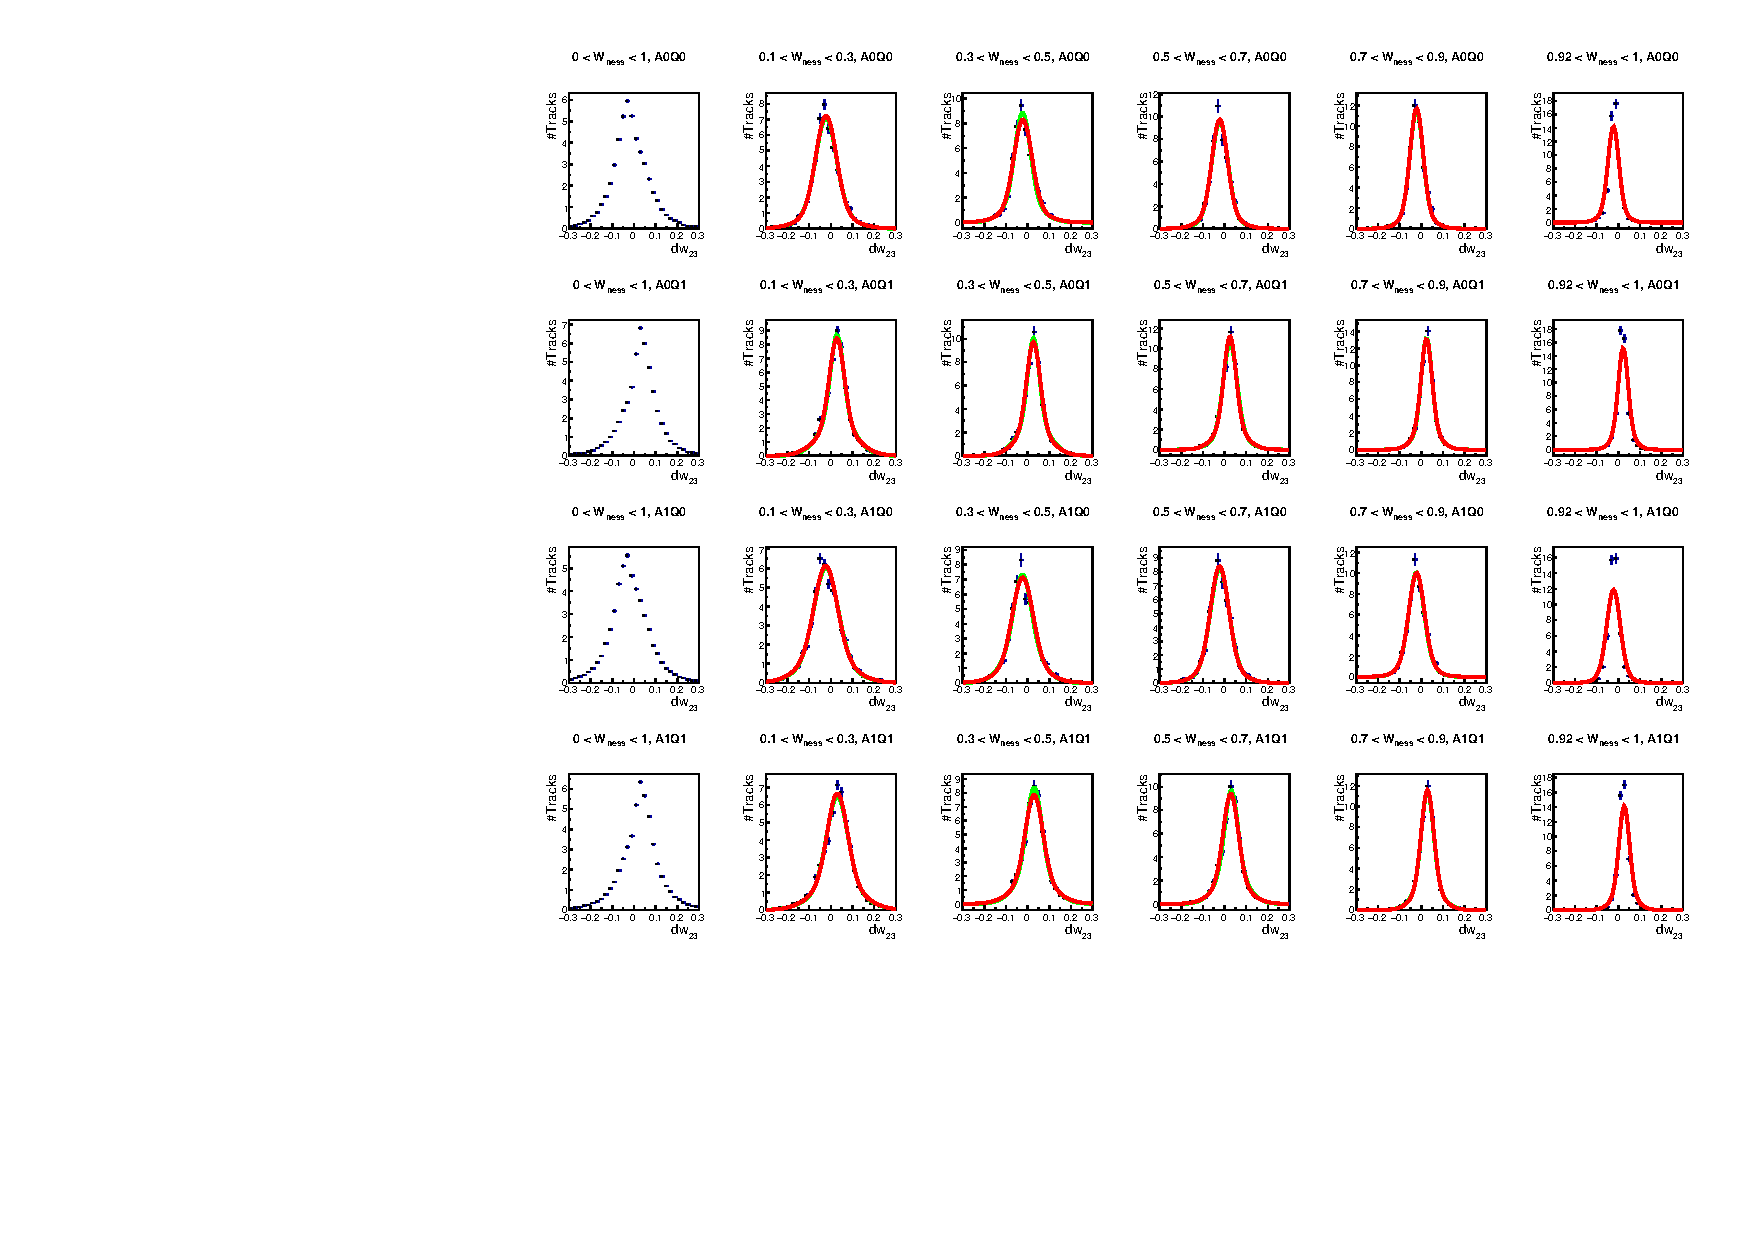
\includegraphics[width=\linewidth]{./figures/dw23_extrap_bins.pdf}
  \caption{
    From left to right the columns show $dw_{23}$ for the full $W_{ness}$ range,
    $0.1 < W_{ness} < 0.3$, $0.3 < W_{ness} < 0.7$, $0.3 < W_{ness} < 0.7$, $0.7
    < W_{ness} < 0.9$. The columns show the extrapolated shape for $W_{ness} >
    0.95$. The red curve shows the 1D projection of the total 2D
    parameterization of $dw_{23}$ vs $W_{ness}$ plotted on top of the green
    curves. The green curve shows the coaxial double Gaussian fit to a slice of
    $dw_{23}$ in $W_{ness}$. The final column shows the projected shape of
    $dw_{23}$ against the signal data region ($W_{ness} > 0.95$). A0 and A1
    refer to North or South arms, Q0 and Q1 refer to negatively or positively
    charged muons.
  }
  \label{fig:dw23_slice_fits}
\end{figure}

\begin{figure}[ht]
  \centering
  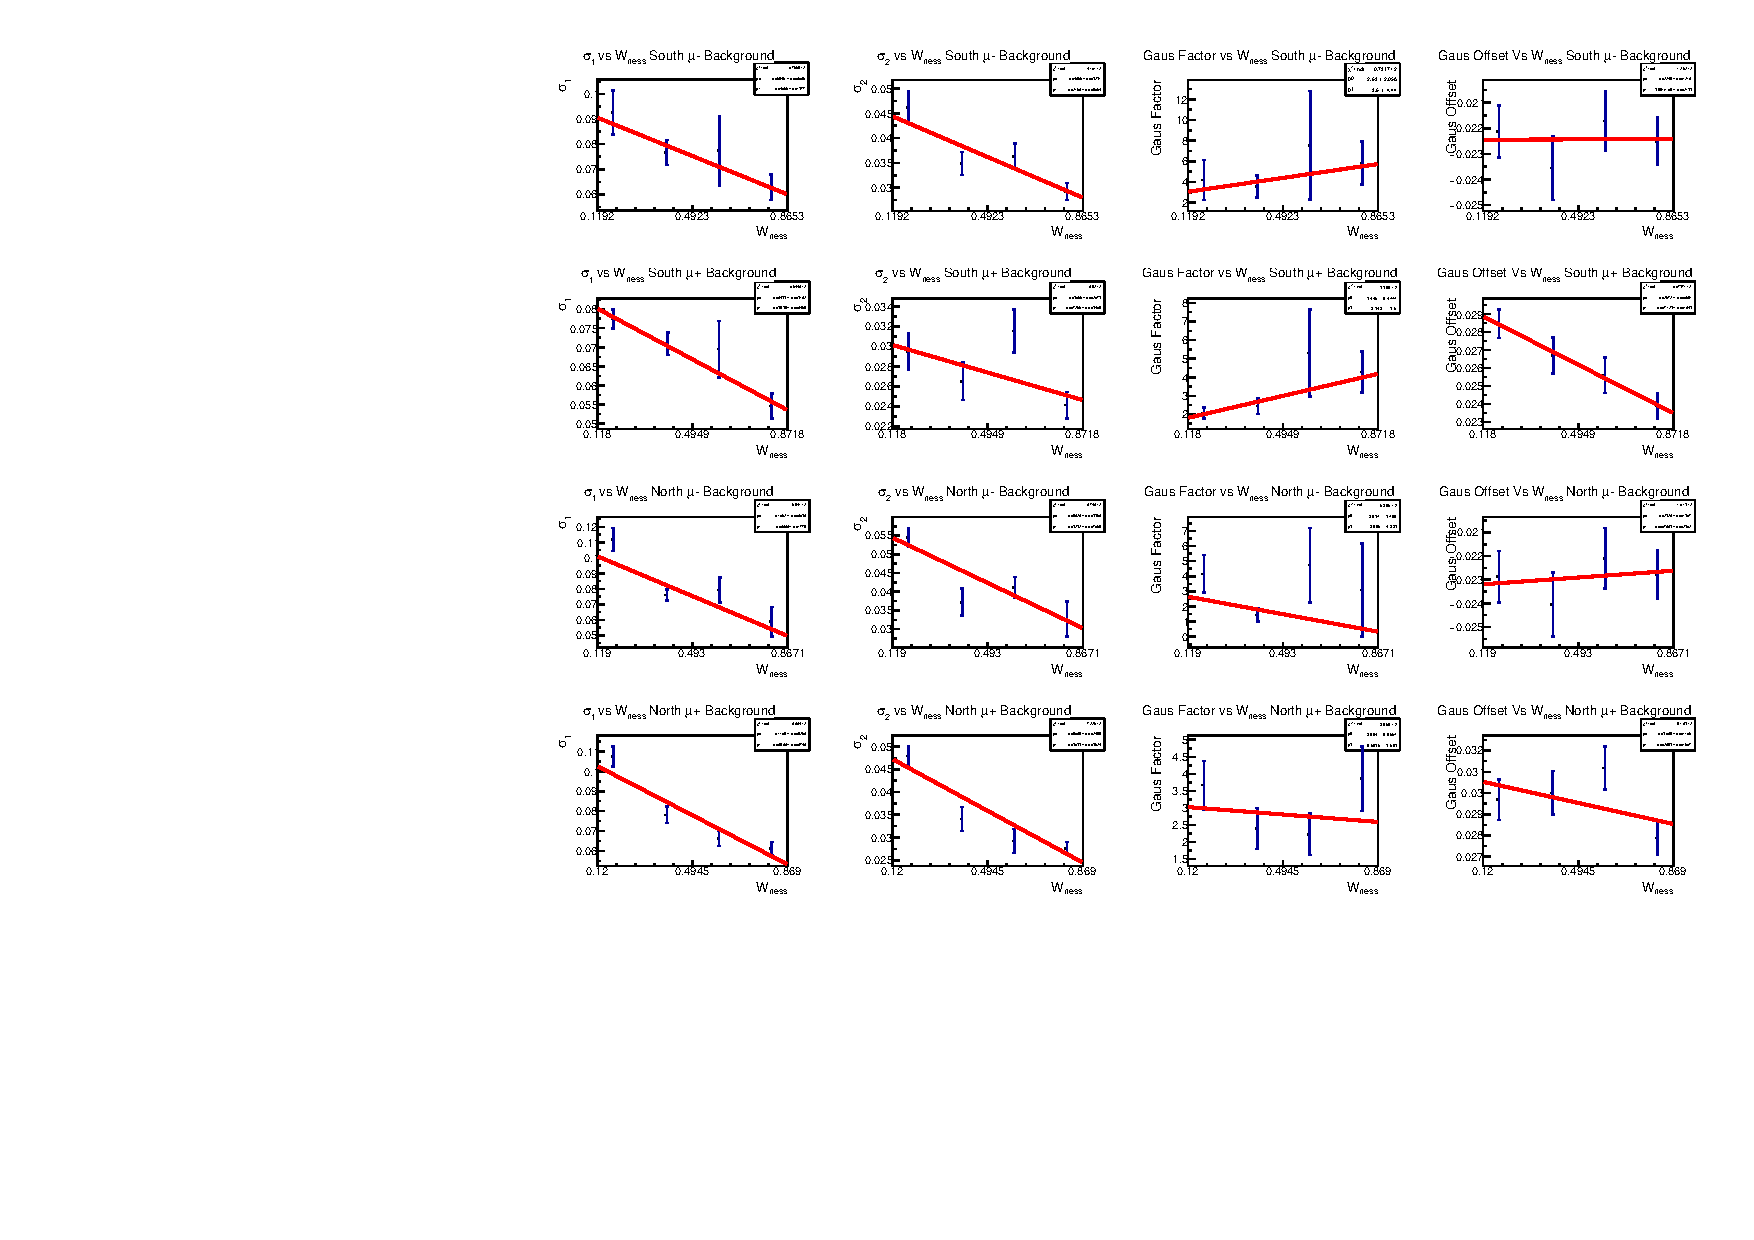
\includegraphics[width=\linewidth]{./figures/dw23_parameters_linearized.pdf}
  \caption{
    The four parameters from the co-axial Gaussian parameterization of $dw_{23}$
    as a function of $W_{ness}$.  Rows are arm/charge, labeled on the left,
    while columns are co-axial Gaussian parameters, summarized in
    Equation~\ref{eq:dw23_parameterization}
  }
  \label{fig:coax_params_vs_wness}
\end{figure}

A full parameterization of $dw_{23}$ as a function of $W_{ness}$ is achieved by
fitting the 2D data set of track-yield vs $dw_{23}$ and $W_{ness}$ with a
two-dimensional function. While the width of $dw_{23}$ as a function of
$W_{ness}$ has been shown to be well described as a coaxial double Gaussian,
whose parameters depend linearly on $W_{ness}$, the overall height of the
distribution must be parameterized as well. The shape of the $W_{ness}$
histogram shown in Figures~\ref{fig:dw23_eta_wness_dat}
and~\ref{fig:dw23_eta_wness_sim} suggests a quartic parameterization. The
$W_{ness}$ distributions are fit, results shown in Figure~\ref{fig:wness_pol4}.

\begin{figure}[ht]
  \centering
  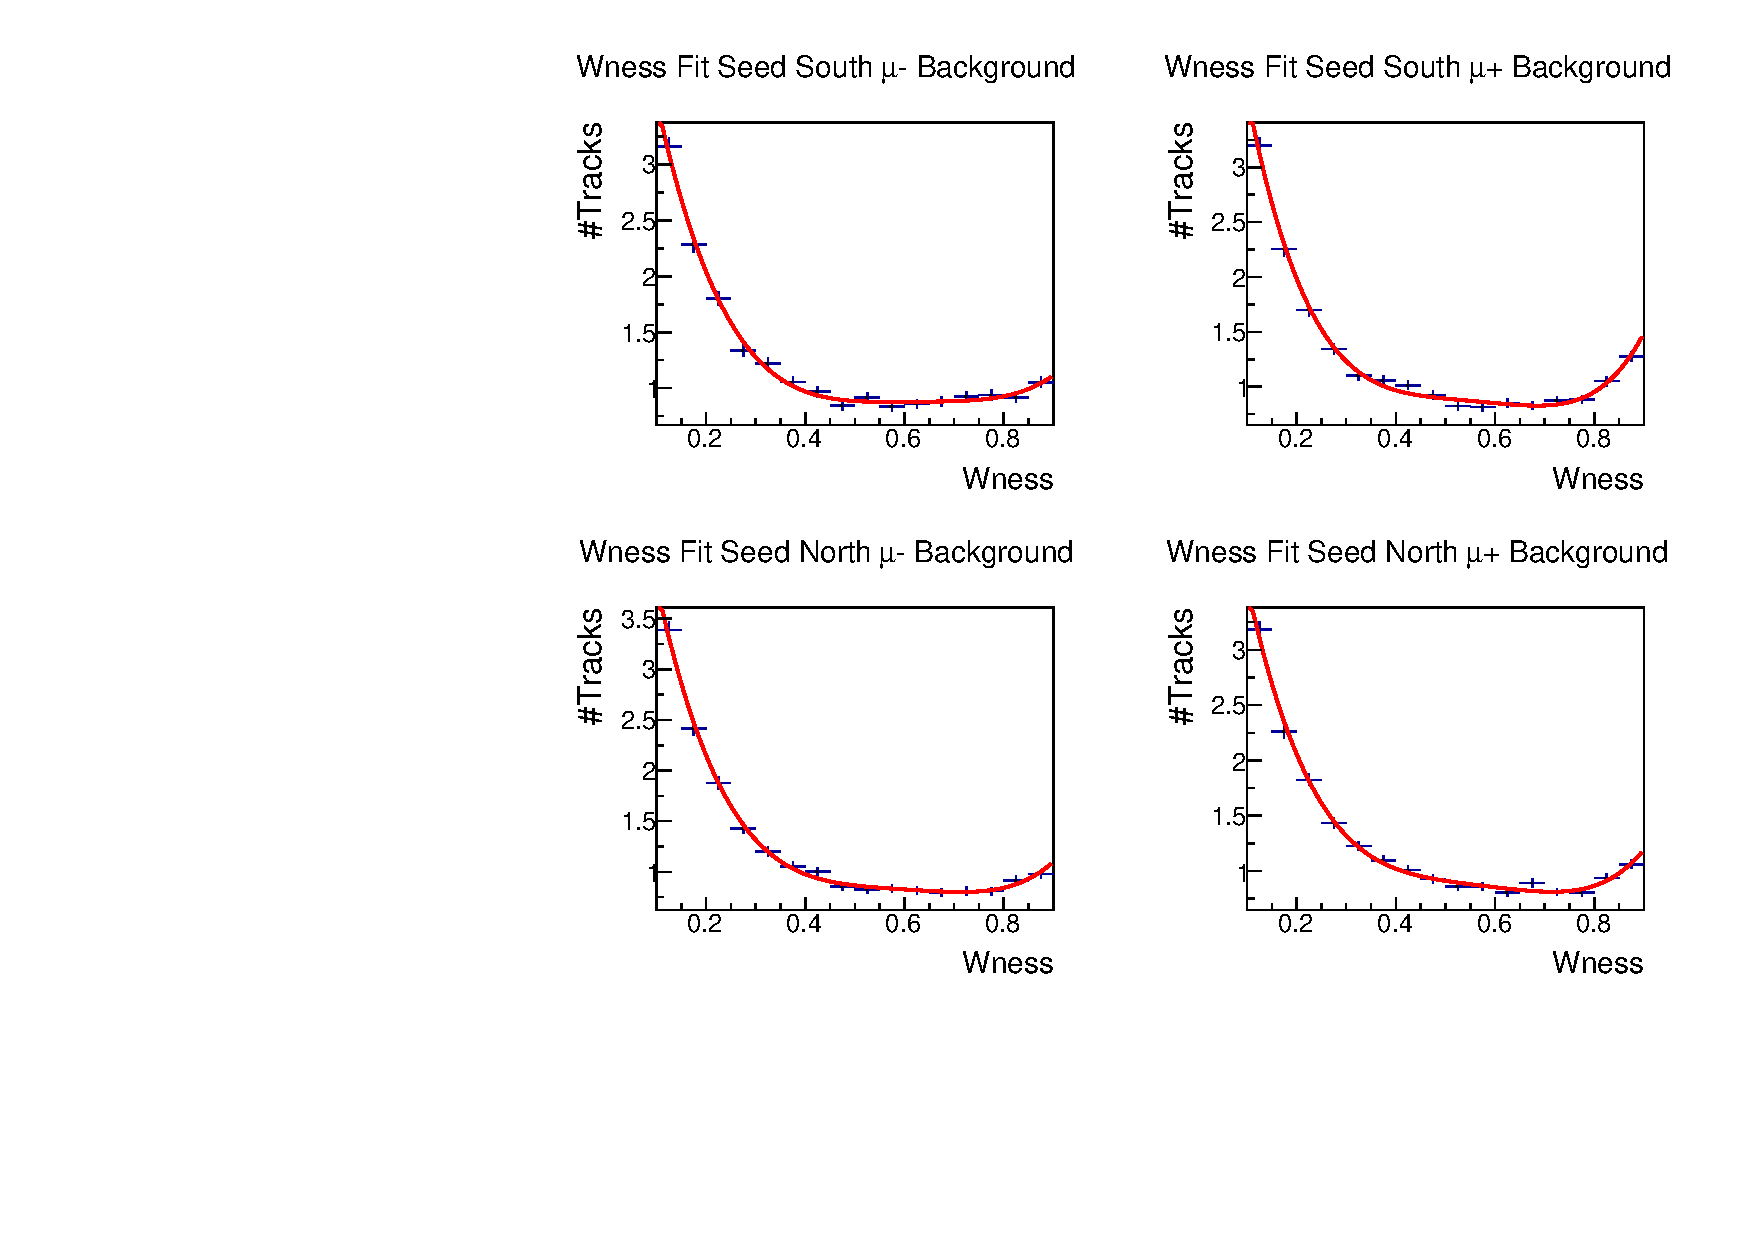
\includegraphics[width=0.7\linewidth]{./figures/c_WnessFit1D.pdf}
  \caption{
    Shown: resulting fourth degree polynomial fit to the yield vs $W_{ness}$
    representing the hadronic background region $0 < W_{ness} < 0.9$ of the real
    data.
  }
  \label{fig:wness_pol4}
\end{figure}

\clearpage
\subsubsection{Final Parameterization of $dw_{23}$}

With reasonable parameterization of our $dw_{23}$ parameter as a function of
$W_{ness}$, a 2D fit is performed which captures both the quartic dependence of
the data set yield vs $W_{ness}$ and the $dw_{23}$ width dependence on
$W_{ness}$.

{\noindent} The parameterization separated into quartic and coaxial Gaussian
potions:

\begin{equation}
  F(W_{ness},dw_{23}) = f(W_{ness})\times g(W_{ness},dw_{23}) 
  \label{eq:dw23_final_parameterization}
\end{equation}

{\noindent}$f(W_{ness})$ represents the fourth-degree polynomial dependence of
yield vs $W_{ness}$:

\begin{equation} \label{eq:wness_pol4}
  f(W_{ness}) = 
  P_8 + P_9 W_{ness} + 
  P_{10} {W_{ness}}^2 +
  P_{11} + {W_{ness}}^3 +
  P_{12} + {W_{ness}}^4
\end{equation}

{\noindent}and $g(W_{ness},dw_{23})$ represents the changing width of the
$dw{23}$ coaxial double Gaussian as a function of $W_{ness}$. The Parameters of
the co-axial double Gaussian to vary linearly with $W_{ness}$:

\begin{align}\label{eq_dw23_equations}
  \sigma_1 &= P_1 + P_3 \times W_{ness} &  C_g &= P_6 + P_7 \times W_{ness} \\
  \sigma_2 &= P_4 + P_5 \times W_{ness} &  \mu &= P_0 + P_1 \times W_{ness}
\end{align}

{\noindent}with $g(W_{ness},dw_{23})$ parameterized:

\begin{equation}
  g(W_{ness},dw_{23}) = C_w \times 
  \left(
    \left( 
      { {1}\over{\sqrt{2\pi}\sigma_1+C_g\sqrt{2\pi}\sigma_2} }
    \right) 
    \times
    \left(
      e^{{{1}\over{2}}{\left({dw_{23-\mu}}\over{\sigma_1}\right)^2}}
        +C_ge^{{{1}\over{2}}{\left({dw_{23-\mu}}\over{\sigma_2}\right)^2}} 
    \right) 
  \right)
  \label{eq:dw23_parameterization}
\end{equation}

The full fit, (Eqtn. ~\ref{eq:dw23_final_parameterization}) is seeded using the
parameters extracted from the 1D slices of $dw_{23}$ in $W_{ness}$. The results
of this fitting procedure are summarized in Figure~\ref{fig:dw23_fits}.

\begin{figure}[ht]
  \centering
	\begin{subfigure}[t]{0.5\textwidth}
		\centering
    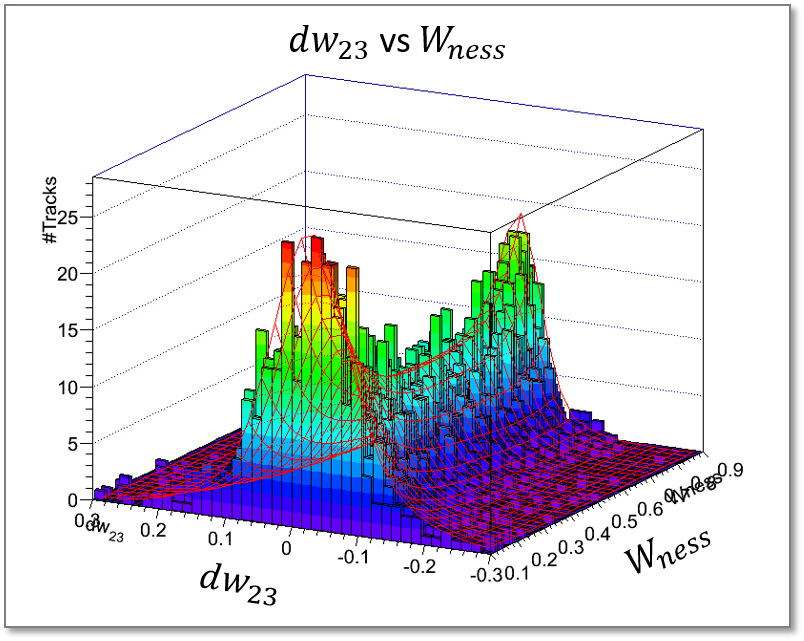
\includegraphics[width=0.95\linewidth]{./figures/dw23_vs_eta_3D.png}
    \caption{The final fit to $dw_{23}$ vs $W_{ness}$}
		\label{fig:3Ddw23_wness}
	\end{subfigure}%
  \begin{subfigure}[t]{0.5\textwidth}
		\centering
		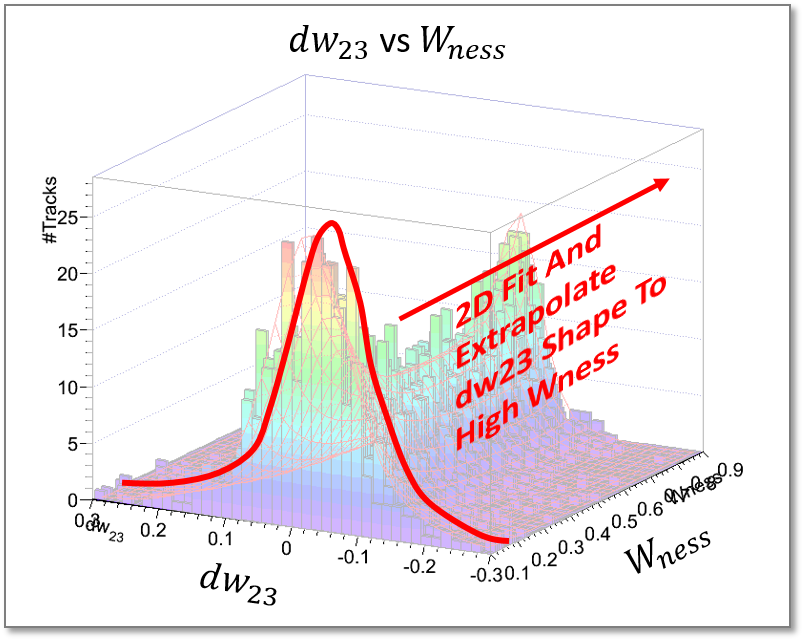
\includegraphics[width=0.95\linewidth]{./figures/dw23_vs_eta_3D_overlay.png}
    \caption{Cartoon of the extrapolation}
		\label{fig:3Ddw23_wness_overlay}
	\end{subfigure}
  \caption{ 
    Panel (a) shows a red wire-frame representing the resultant fit of to the
    $dw_{23}$ vs $W_{ness}$ distribution, against the lego-style real data
    distribution. Panel (b) shows the process of extrapolating the shape of
    $dw_{23}$ from lower $W_{ness}$ to the signal region to obtain the hadronic
    background PDF representing $dw_{23}$.
  }
  \label{fig:dw23_fits}
\end{figure}

Finally, the extrapolation of $dw_{23}$ was reproduced and cross-checked by four
independent analyzers. The distributions are in close agreement:
Figure~\ref{fig:four_dw23}.

\begin{figure}
  \centering
  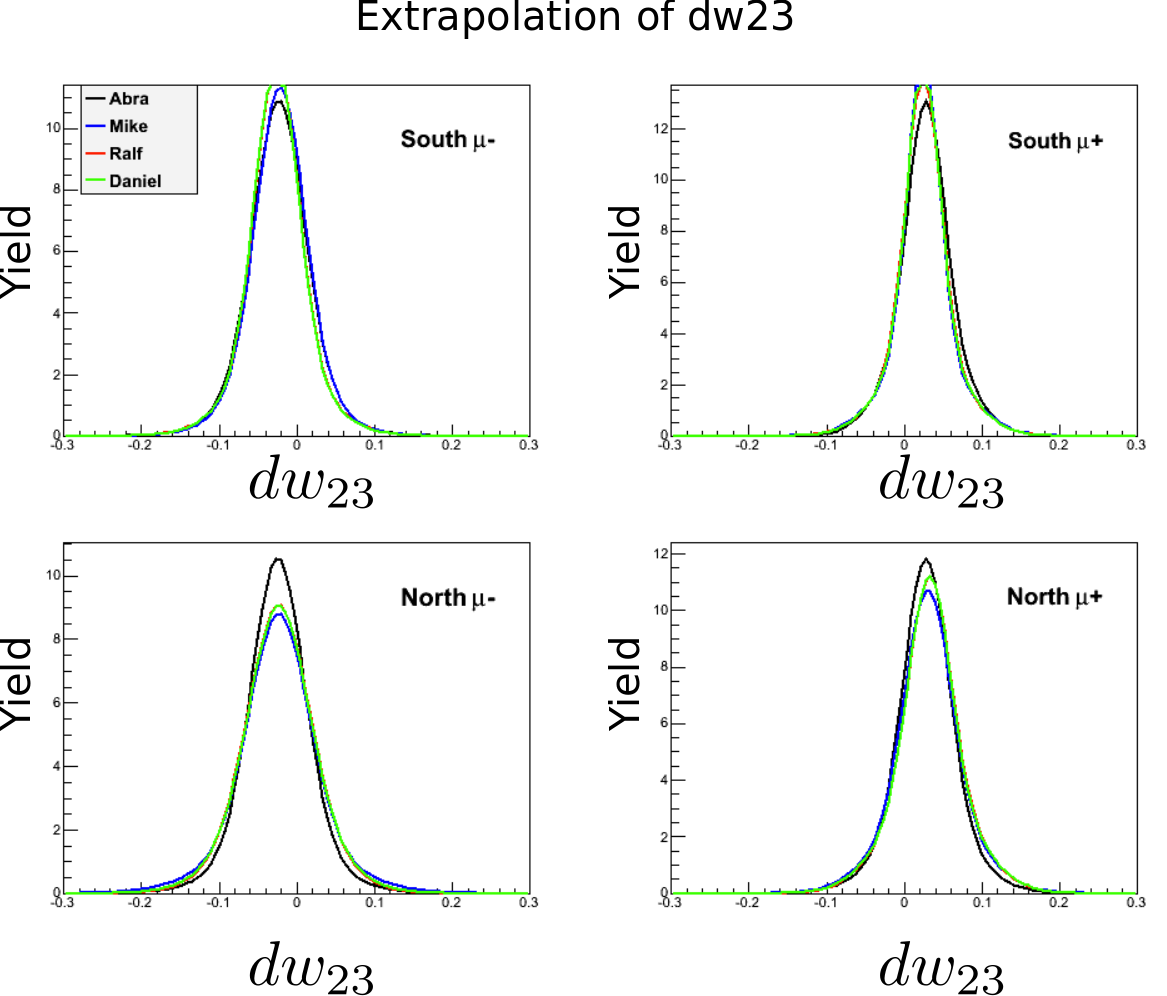
\includegraphics[width=0.7\linewidth]{./figures/dw23_fourway.png}
  \caption{
    Shown: a comparison of four independent extrapolations of $dw_{23}$ into
    the signal region~\cite{Seidl2014a}.
  }
  \label{fig:four_dw23}
\end{figure}

The PDF for the variable $\eta$ representing the hadronic background was
obtained by creating a histogram of the variable for events tagged with
$W_{ness} < 0.9$. 

\clearpage
\subsection{Muon Background and W-Signal PDFs}
\label{sec:simulation_pdfs}


Simulations are used to define the distributions $dw_{23}$ and $\eta$, for PDFs
representing both $W$ signal and Muon Background processes.

As discussed in Section~\ref{sec:simulations} and in the introduction to this
Section (\ref{sec:sbr_intro}), the Muon Background is modeled with simulations,
which are summed to a representative PDF by scaling the simulated yields to
match what is expected in the data set. Since the $W$ signal is singular in
source, no scaling is needed, as the PDFs are normalized before being used in
any calculation.

\subsubsection{Multiple Collisions and Pile-Up}

Simulations are produced using a reference run as a means of comparison. In the
case of this analysis, the reference run used to seed simulations is 393888.

When events are generated for each muon process and added, they must be weighted
for luminosity, cross section, k-factor and generated events to get an overall
factor with which weight each individual distribution to generate the total
`Muon Background' distributions. For event generation, one must sum to obtain a
sample consistent with the PHENIX sampled luminosity of $277 pb^{-1}$, which has
been corrected for pile-up and multiple collisions.

The pile-up correction has been performed for all three $W\rightarrow\mu$
and closely follows the procedure most recently detailed in ~\cite{Wolin2014}.
For our luminosity detector, the BBC, one must consider that the BBC has a
finite efficiency for the North and South subsystems, and therefore can
mis-count the actual number of collisions.

Instead of calculating the efficiencies for a finite number of collisions in
one crossing, it is easier to calculate the probability of not counting
any collision. In an iterative procedure which generally converges after one or
two iterations, the north (south) efficiencies $k_N$, ($k_S$) were evaluated
based on the true number of collisions per crossing $\mu$:

\begin{equation}
  R_{BBC} = 1 - e^{-\mu\epsilon_{BBC}(1+k_N)} - 
  e^{-\mu\epsilon_{BBC}(1+k_S)} + 
  e^{-\mu\epsilon_{BBC}(1+k_N+k_S)}\quad,
\end{equation}

{\noindent}where $R_{BBC}$ is the observed number of collisions per crossing and
$\epsilon_{BBC}$ is the overall BBC efficiency of 0.53, describing the fraction
of the time the BBC will trigger on event, given that an event has occurred.

This way the actual average collisions rate can be evaluated for each run and
the actual luminosity can then be obtained via the collision frequency (
$f_{coll} = 1/(106 ns)$), the length of a run $t$,  and its live fraction and
the total BBC cross section ( at 510 GeV: $\sigma_{pp} = 61$ mb ):

\begin{equation}
  L_i = \frac{BBC_{live}}{ BBC_{raw}} 
  \times t \times f_{coll} / 
  \sigma_{pp}\quad . 
\end{equation}

Summing up all produced runs available, one obtains a total luminosity of 277
pb$^{-1}$. 

The actual number or collisions as well as the measured and true minimum bias
collisions rates for each run are displayed in Fig.~\ref{fig:bbc_mc}. One sees,
that on average one has 0.74 collisions per crossing which motives the reference
run (393888) selection for the simulation, since this run had the same average
collision rate.

\begin{figure}
  \centering
  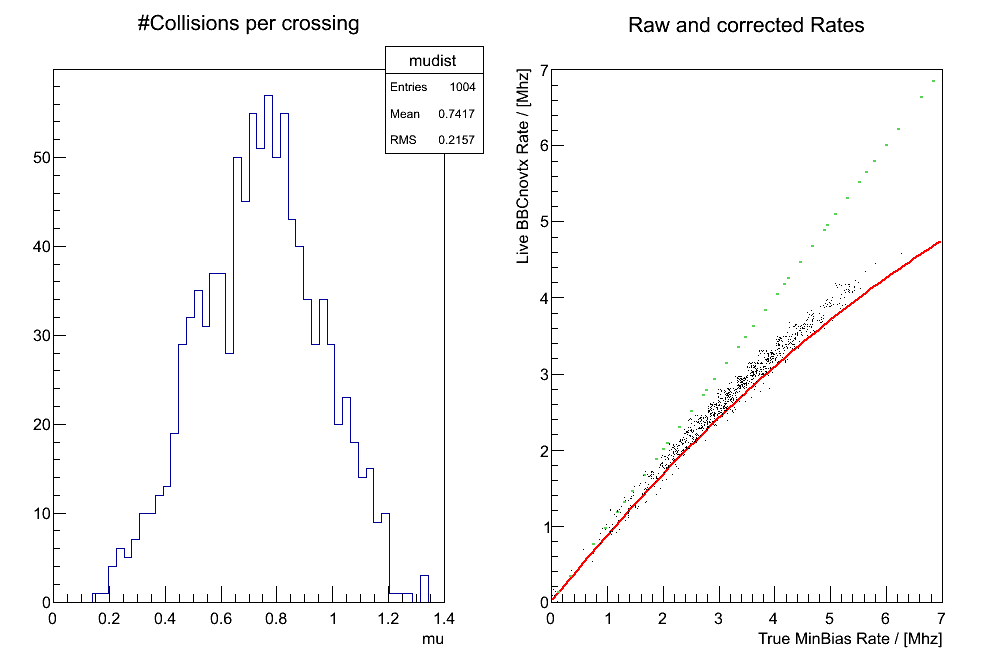
\includegraphics[width=0.9\linewidth]{./figures/BBCrawcorrrates2.png}
  \caption{
    Left: distribution of number of collisions per crossing $\mu$ for all runs
    available from the  2013 data set. Right: True and observed BBCnovtx live
    rates for all runs as a function of the true rate and calculated as
    described in the text. The green, dashed line represents a perfect
    accounting of true collisions, while the red curve takes the efficiencies of
    the two BBC sides into account~\cite{Seidl2014a}.
  }
  \label{fig:bbc_mc}
\end{figure}

\clearpage
\subsection{Final PDFs Used in EULMF}

The PDFs which were used in the EULMF are summarized in Figures
\ref{fig:c_dw23_Eta_PDF_Arm0_Charge0}-\ref{fig:c_dw23_Eta_PDF_Arm1_Charge1}. The
PDFs have been smoothed with a moving windowed-average algorithm to remove
statistical fluctuations, with the overall shape apparently different for
Hadronic Background, Muon Background and $W$ signal. $dw_{23}$, as expected, has
the narrowest distribution for the $W$ signal PDFs, with the broadest width for
the hadronic background. 

\begin{figure}
  \centering
  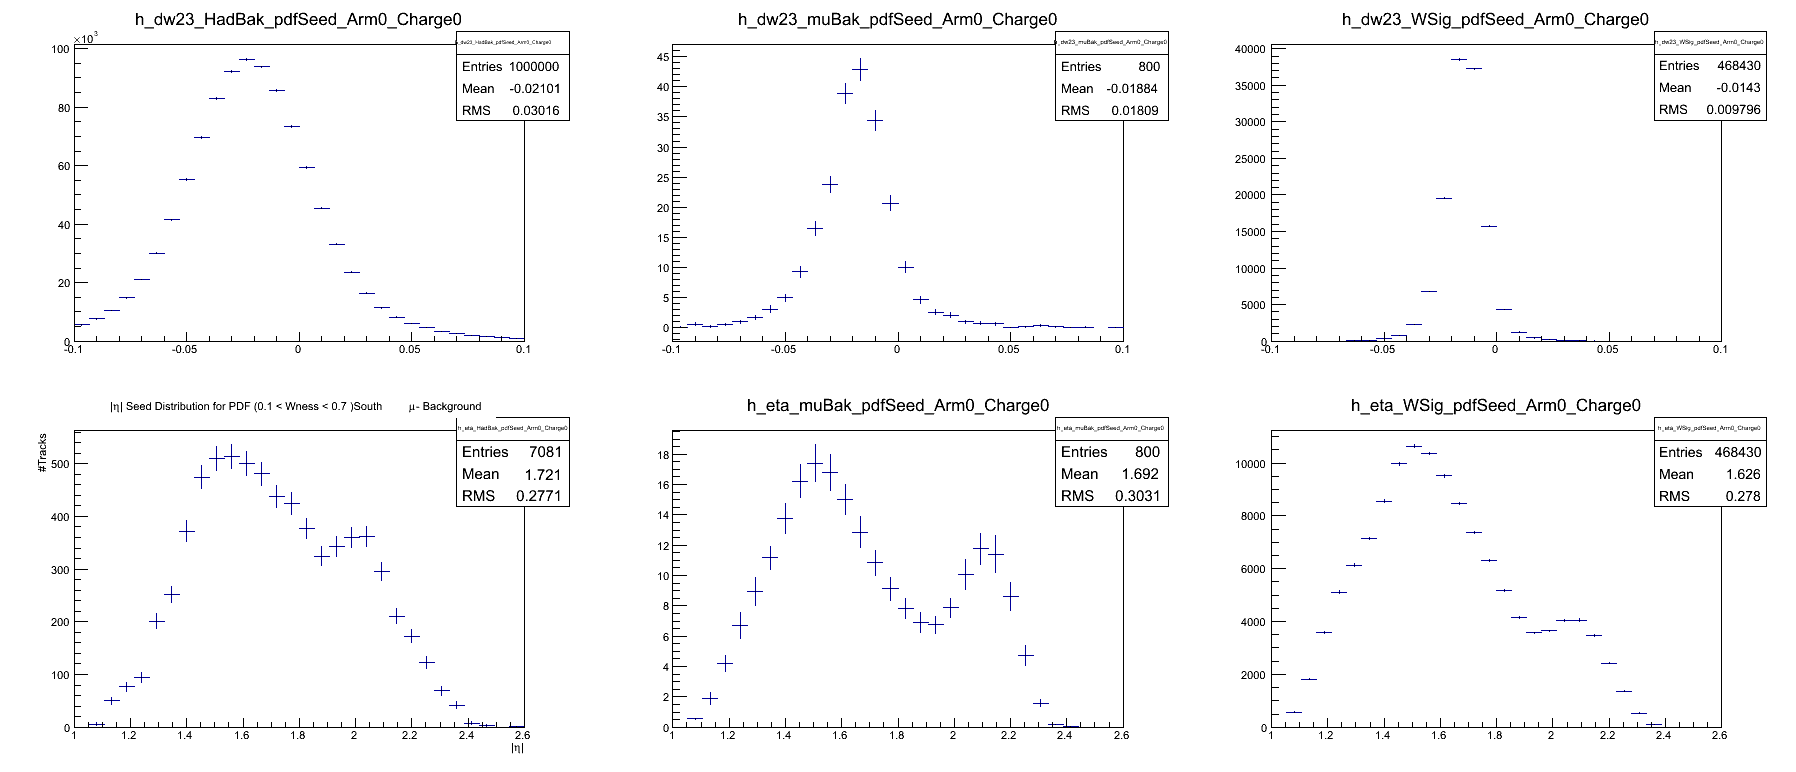
\includegraphics[width=\linewidth]{./figures/c_dw23_Eta_PDF_Arm0_Charge0.png}
  \caption{
    Left Column: The hadronic background PDFs, Middle Column: The Summed Muon
    Background PDFs, Right Column: The W-Signal PDF. For South Arm, $\mu+$
  }
  \label{fig:c_dw23_Eta_PDF_Arm0_Charge0}
\end{figure}

\begin{figure}
  \centering
  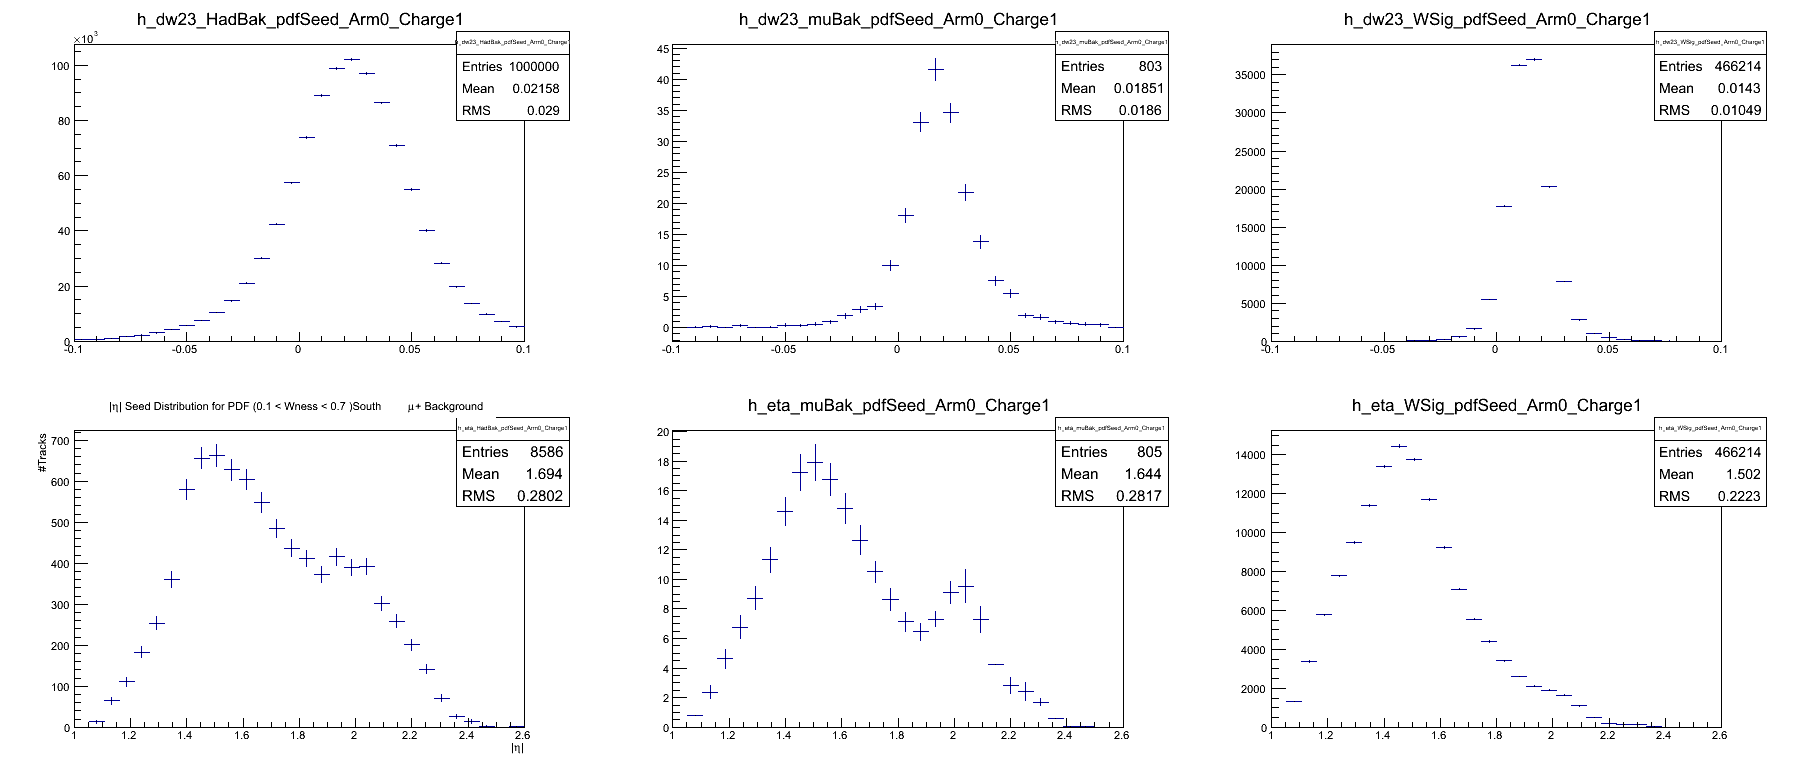
\includegraphics[width=\linewidth]{././figures/c_dw23_Eta_PDF_Arm0_Charge1.png}
  \caption{
    Left Column: The hadronic background PDFs, Middle Column: The Summed Muon
    Background PDFs, Right Column: The W-Signal PDF. For South Arm, $\mu-$
  }
  \label{fig:c_dw23_Eta_PDF_Arm0_Charge1}
\end{figure}

\begin{figure}
  \centering
  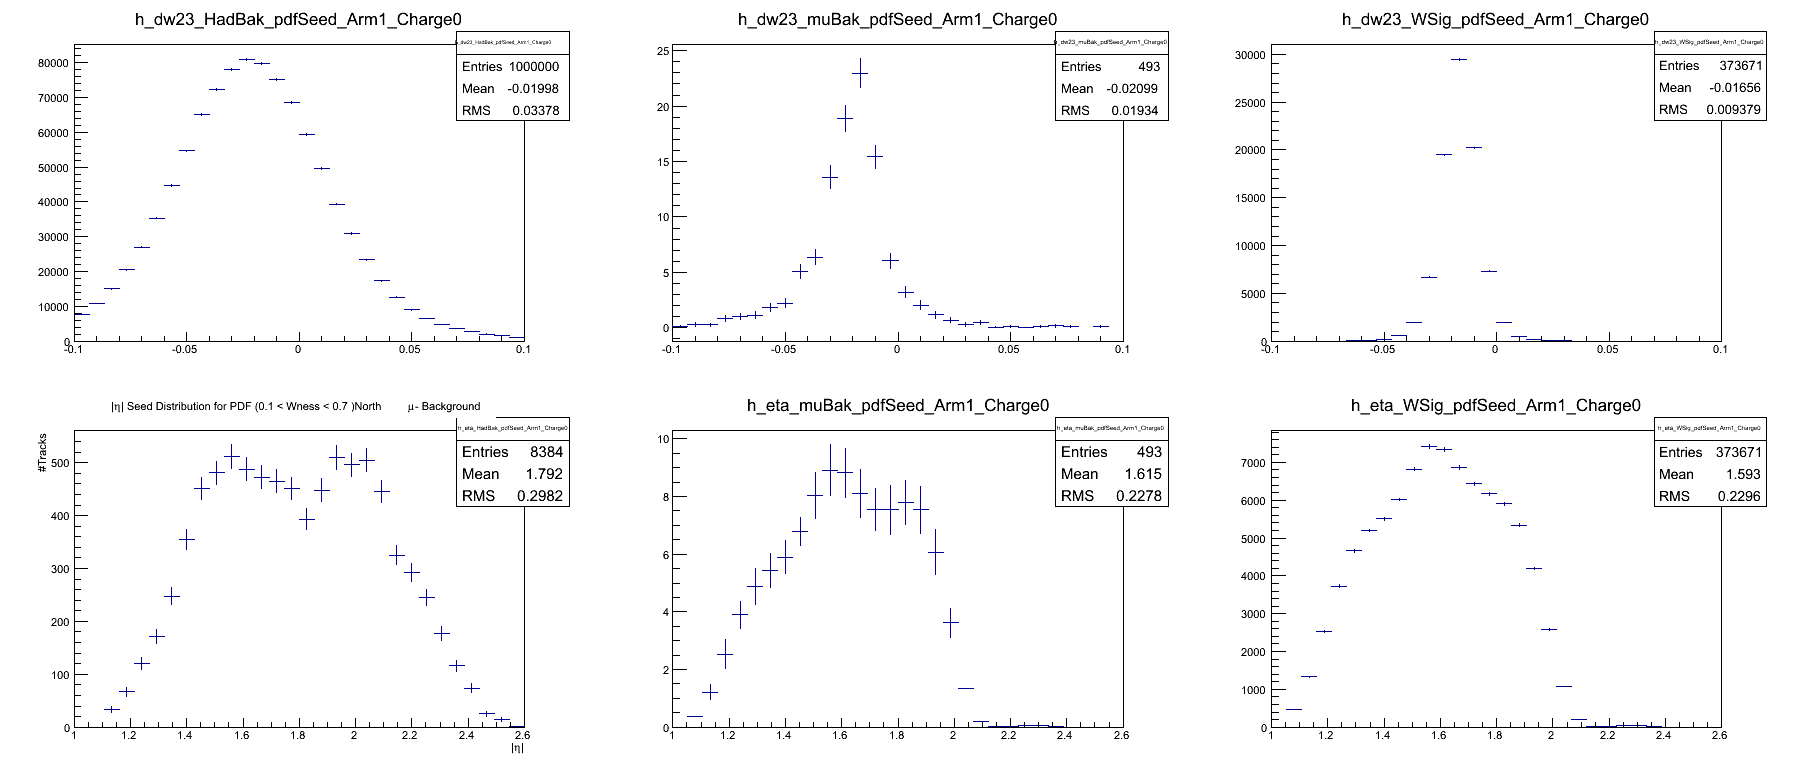
\includegraphics[width=\linewidth]{././figures/c_dw23_Eta_PDF_Arm1_Charge0.png}
  \caption{
    Left Column: The hadronic background PDFs, Middle Column: The Summed Muon
    Background PDFs, Right Column: The W-Signal PDF. For North Arm, $\mu-$
  }
  \label{fig:c_dw23_Eta_PDF_Arm1_Charge0}
\end{figure}

\begin{figure}
  \centering
  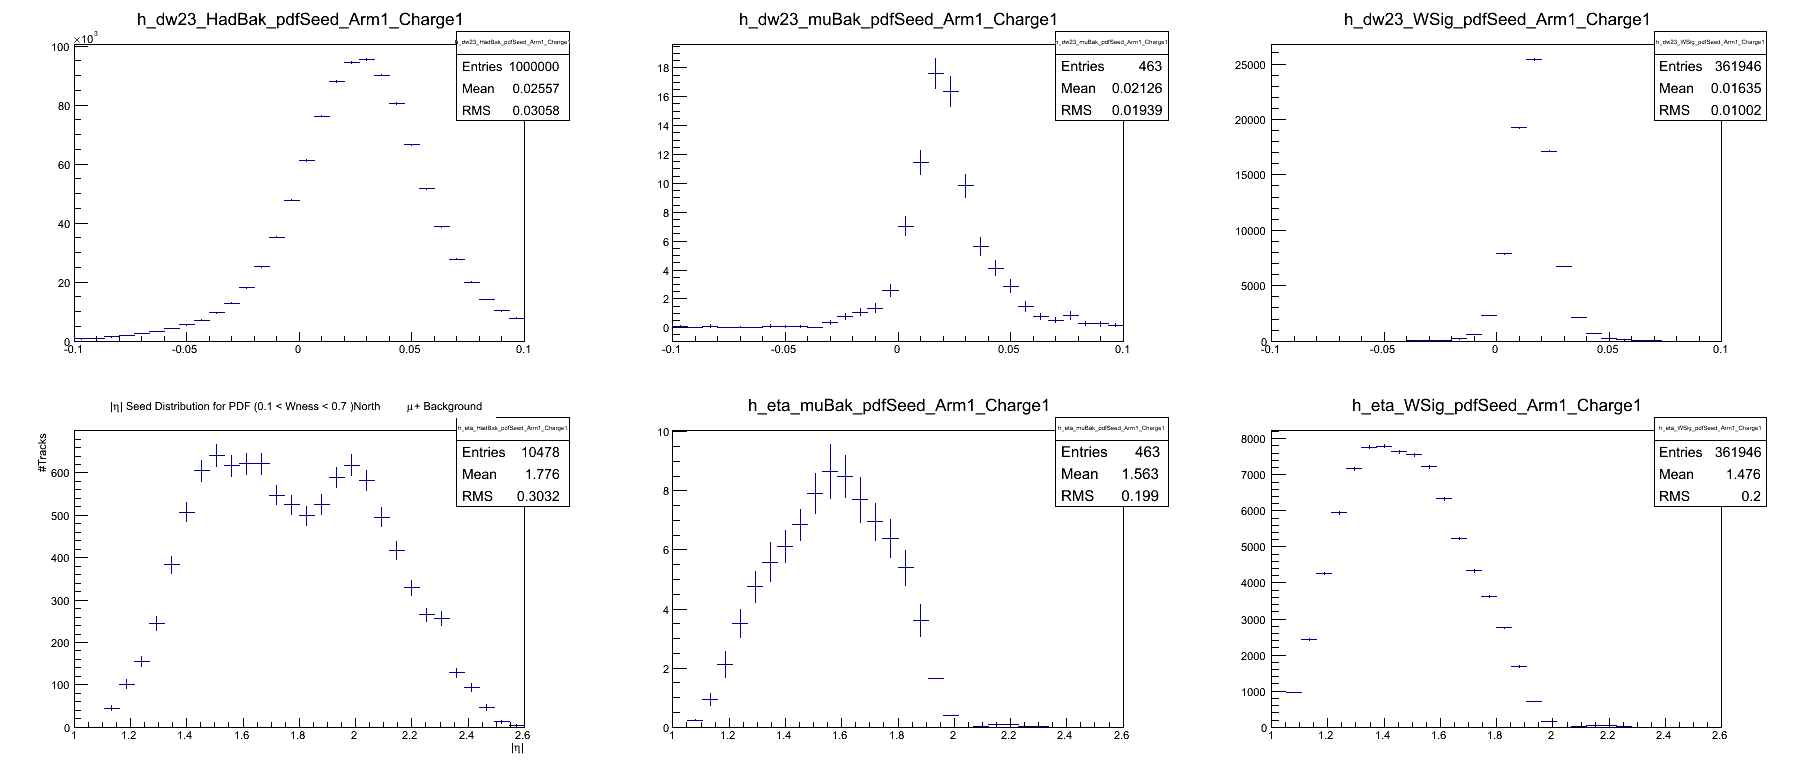
\includegraphics[width=\linewidth]{././figures/c_dw23_Eta_PDF_Arm1_Charge1.png}
  \caption{
    Left Column: The hadronic background PDFs, Middle Column: The Summed Muon
    Background PDFs, Right Column: The W-Signal PDF. For South Arm, $\mu+$
  }
  \label{fig:c_dw23_Eta_PDF_Arm1_Charge1}
\end{figure}

\clearpage
\subsubsection{EULMF Fit Results}

With all PDFs prepared, the EULMF is executed, and the resultant yields for the
Hadronic Background + Muon Background (which was fixed) and the $W$ signal are
obtained. From these yields, the signal to background ratios with associated
uncertainties are estimated. The results of the EULMF are shown in
Figures~\ref{fig:maxlikefit_a0q0}-\ref{fig:maxlikefit_a1q1}.

\begin{figure}[ht]
  \centering
  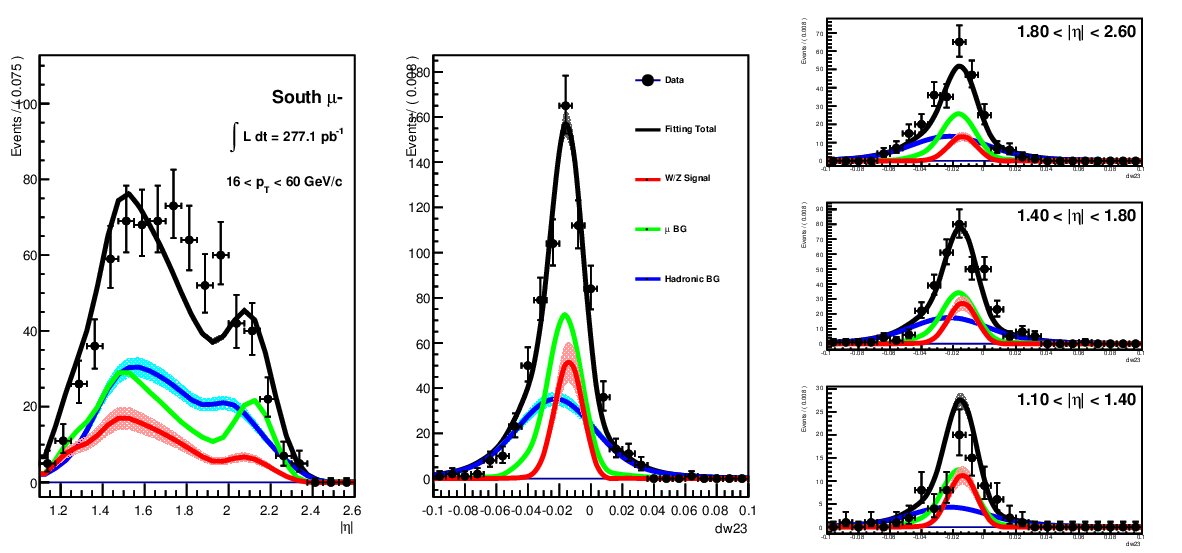
\includegraphics[width=\linewidth]{./figures/prelim_full_maxlikefit_a0q0.jpg}
  \caption{
    Here, we see the preliminary results of the EULMF for the 2013 Run. On the
    left, $\eta$ is shown. In the middle, $dw_{23}$. On the right, $dw_{23}$ is
    subdivided into the three standard $\eta$ bins. In all cases, we see the
    unbinned data in black (with error bars), and the sum of the three fits in
    black. In Blue, we can see the fake-muon hadronic background. In Green, the
    muon background. In blue, we see the W-Signal result. The area under the
    curves represents the yield, relative to the total. Shown: South Arm,
    $\mu-$~\cite{Seidl2014a}
  }
  \label{fig:maxlikefit_a0q0}
\end{figure}

\begin{figure}[ht]
  \centering
  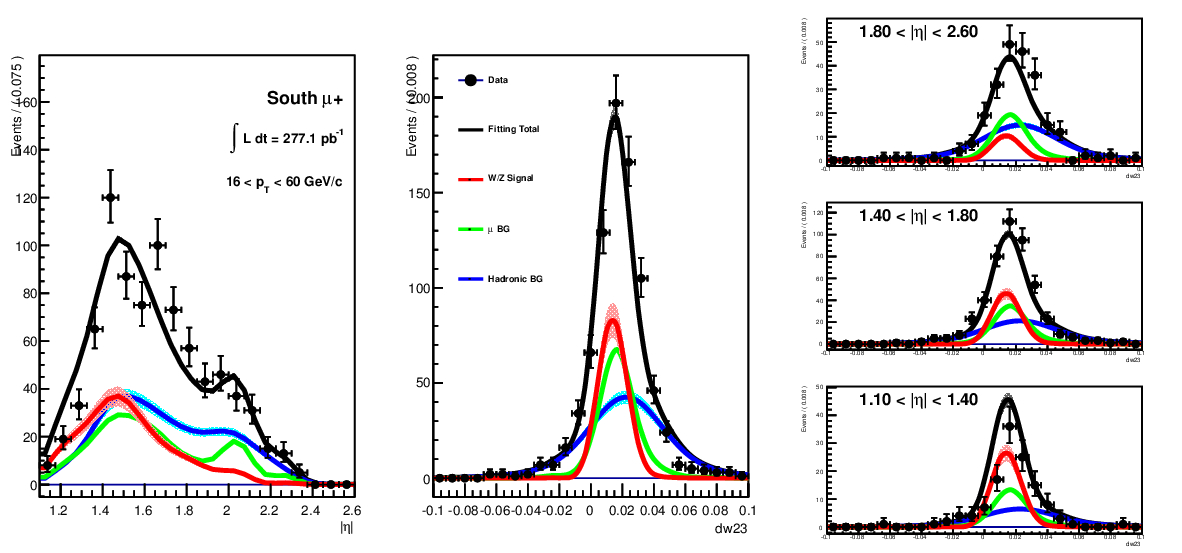
\includegraphics[width=\linewidth]{./figures/prelim_full_maxlikefit_a0q1.jpg}
  \caption{
    Here, we see the preliminary results of the EULMF for the 2013 Run. On the
    left, $\eta$ is shown. In the middle, $dw_{23}$. On the right, $dw_{23}$ is
    subdivided into the three standard $\eta$ bins. In all cases, we see the
    unbinned data in black (with error bars), and the sum of the three fits in
    black. In Blue, we can see the fake-muon hadronic background. In Green, the
    muon background. In blue, we see the W-Signal result. The area under the
    curves represents the yield, relative to the total.  Shown: South Arm,
    $\mu+$~\cite{Seidl2014a}
  }
  \label{fig:maxlikefit_a0q1}
\end{figure}

\begin{figure}[ht]
  \centering
  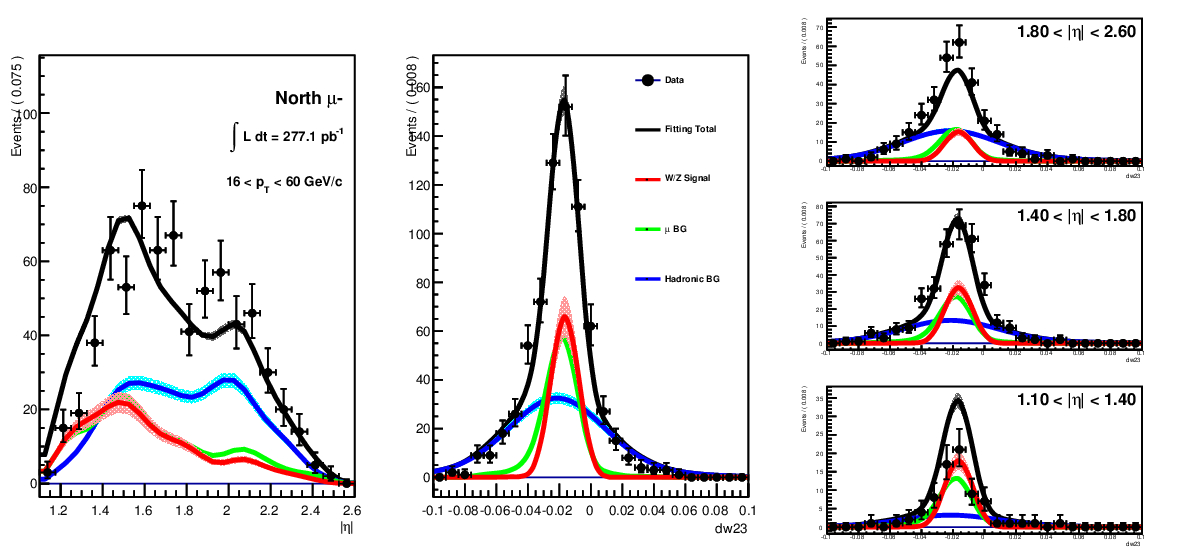
\includegraphics[width=\linewidth]{./figures/prelim_full_maxlikefit_a1q0.jpg}
  \caption{
    Here, we see the preliminary results of the EULMF for the 2013 Run. On the
    left, $\eta$ is shown. In the middle, $dw_{23}$. On the right, $dw_{23}$ is
    subdivided into the three standard $\eta$ bins. In all cases, we see the
    unbinned data in black (with error bars), and the sum of the three fits in
    black. In Blue, we can see the fake-muon hadronic background. In Green, the
    muon background. In blue, we see the W-Signal result. The area under the
    curves represents the yield, relative to the total.  Shown: North Arm,
    $\mu-$~\cite{Seidl2014a}
  }
  \label{fig:maxlikefit_a1q0}
\end{figure}

\begin{figure}[ht]
  \centering
  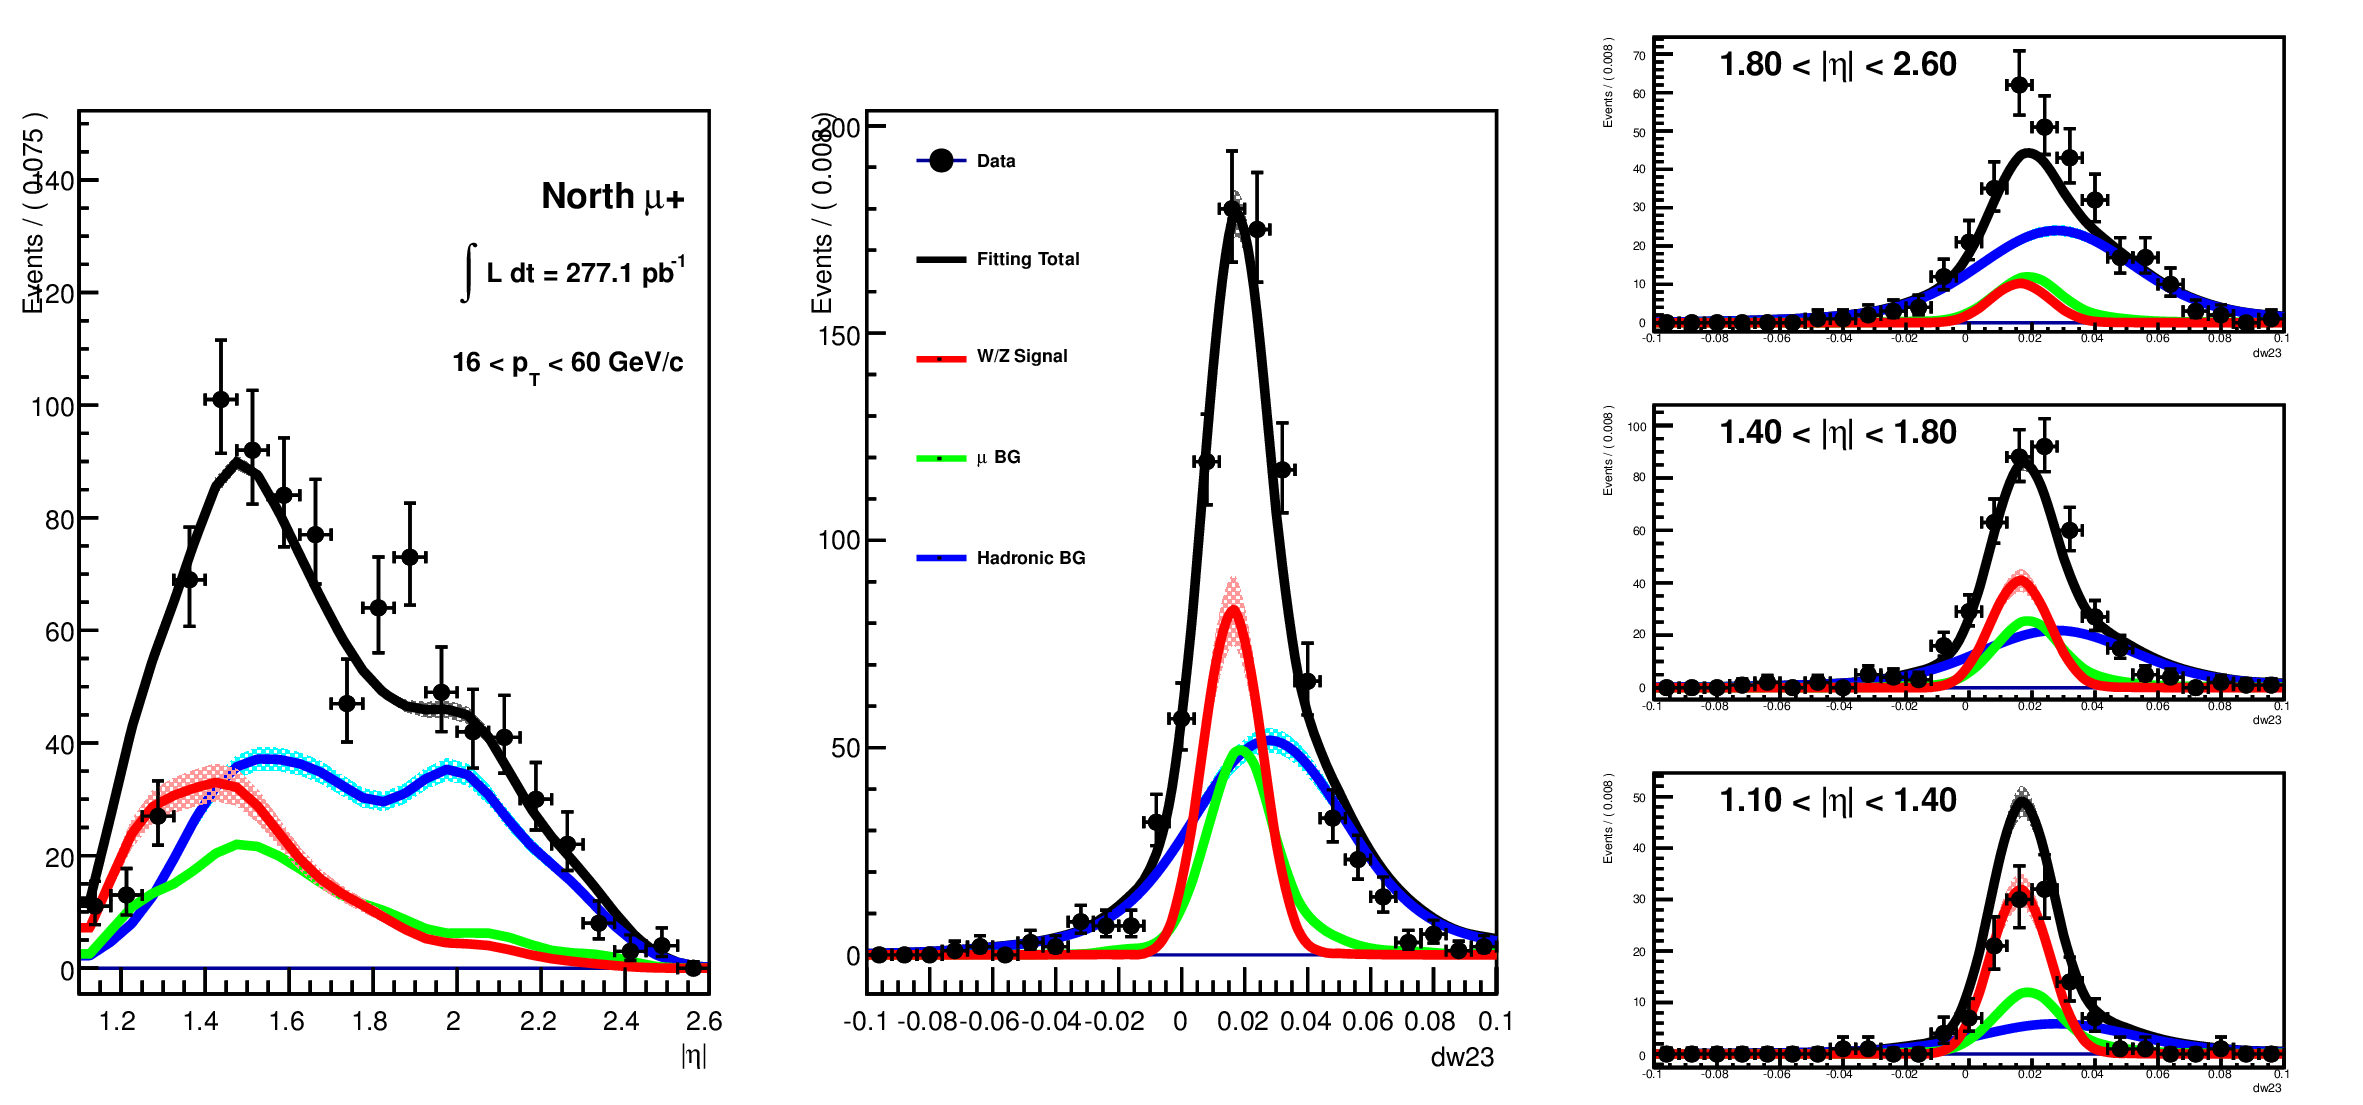
\includegraphics[width=\linewidth]{./figures/prelim_full_maxlikefit_a1q1.jpg}
  \caption{
    Here, we see the preliminary results of the EULMF for the 2013 Run. On the
    left, $\eta$ is shown. In the middle, $dw_{23}$. On the right, $dw_{23}$ is
    subdivided into the three standard $\eta$ bins. In all cases, we see the
    unbinned data in black (with error bars), and the sum of the three fits in
    black. In Blue, we can see the fake-muon hadronic background. In Green, the
    muon background. In blue, we see the W-Signal result. The area under the
    curves represents the yield, relative to the total. Shown: North Arm,
    $\mu+$~\cite{Seidl2014a}.
  }
  \label{fig:maxlikefit_a1q1}
\end{figure}

The signal to background ratio extraction is summarized and cross-checked among
four independent analyses of the recorded data set. Each analyzer's result is
presented alongside my result in Table~\ref{tab:sbr_per_analyzer}, for the South
Arm $\mu-$ (the canonical cross check, among the analyzers).

\begin{table}[ht]
  \centering
  \resizebox{\textwidth}{!}{\begin{tabular}{c|rrrr}
      \toprule
      \multicolumn{5}{c}{\textbf{South $\mu ^{-}$}}  \\  
      \textbf{Variable} & \textbf{Ralf} & \textbf{Daniel} & \textbf{Mike} &
      \textbf{Abraham} \\  
      \midrule
      \textbf{Total events} & $    2032$&$    2034$&$     2022$&$     2039$\\ 
      \textbf{Signal events} & $     340^{+42.14} _{-41.42}$&$      303^{+42.31} _{-41.59}$&$      332^{+42.28} _{-41.58}$&$      294^{+41.38} _{-41.38}$\\ 
      \textbf{Hadron events} & $    1424^{+53.57} _{-52.60}$&$     1469^{+54.55} _{-53.59}$&$     1433^{+53.97} _{-52.99}$&$     1485^{+53.85} _{-53.85}$\\ 
      \textbf{Muon events} & $     269$&$     262$&$      257$&$      259$\\  
      \textbf{Signal/BG} & $    0.20^{+0.03} _{-0.03}$&$     0.18^{+0.00} _{-0.00}$&$     0.20^{+0.03} _{-0.03}$&$     0.17^{+0.02} _{-0.00}$\\ 
      \bottomrule
  \end{tabular}}
  \caption{ 
    South arm $W\rightarrow \mu^{-}$ fit results per analyzer
    ~\cite{Seidl2014a}
  }
  \label{tab:sbr_per_analyzer}
\end{table}
\clearpage

For all data partitions, the signal to background ratio is presented in
Table~\ref{tab:fullsbrtable}.

\begin{sidewaystable}[ht]
  \centering
  \resizebox{\textwidth}{!}{\begin{tabular}{llccccc}
      \toprule
      \textbf{Arm} & 
      \textbf{Charge} & 
      \textbf{Total Events} & 
      \textbf{Signal Events} & 
      \textbf{Fake Muons} & 
      \textbf{Muon Background} & 
      \textbf{SBR} \\
      \midrule
      S & $\mu-$ & 2023 & $354^{+41.9714}_{-41.2598}$ & $1448^{53.6777}_{-52.7162}$ & $221^{0.212103}_{0.0263482}$ & 0.0258992 \\
      S & $\mu+$ & 2468 & $498^{+44.0941}_{-43.2297}$ & $1767^{57.046 }_{-56.3006}$ & $203^{0.252792}_{0.0238242}$ & 0.0233755 \\
      N & $\mu-$ & 2029 & $370^{+34.4599}_{-33.7046}$ & $1555^{48.5042}_{-47.6586}$ & $104^{0.223026}_{0.0219055}$ & 0.0214353 \\
      N & $\mu+$ & 2633 & $505^{+37.9628}_{-37.2192}$ & $2043^{54.5676}_{-53.7571}$ & $85 ^{0.237312}_{0.0189323}$ & 0.0185715 \\
      \bottomrule
  \end{tabular}}
  \caption{ 
    A summary table from the results of the EULMF to the unbinned data set,
    summed to one $\eta$ bin per arm and charge.
  }
  \label{tab:fullsbrtable}
\end{sidewaystable}

\clearpage
\section{Systematic Tests}

One of the rare advantages of this analysis was that I had the opportunity to
undertake it in parallel with others, working as a team to accomplish goals.  As
a result, there were many complimentary systematic tests undertaken by others,
summarized in Appendix~\ref{appendix_1}. These tests all confirm that the
standardized checks for systematic problems with the analysis undertaken in many
PHENIX spin analysis,  do not yield any uncertainty to this analysis.  
